\documentclass[12pt, letterpaper]{article}
\usepackage[margin=1in]{geometry}
\usepackage[T1]{fontenc}
\usepackage{lmodern}
\usepackage{cmap}
\usepackage[utf8]{inputenc}
\usepackage{amsmath, amssymb, amsthm}
\usepackage{mathtools}
\usepackage{enumitem}
\usepackage{booktabs}
\usepackage{xcolor}
\usepackage{titlesec}
\usepackage{parskip}
\usepackage{hyperref}
\usepackage{fancyhdr}
\usepackage{tcolorbox}
\usepackage{graphicx}
\usepackage{caption}
\tcbuselibrary{skins, breakable}

\definecolor{darkblue}{RGB}{15,55,115}
\definecolor{midblue}{RGB}{30,100,180}
\definecolor{theorybg}{RGB}{245,250,255}
\definecolor{questionbg}{RGB}{255,252,240}
\definecolor{evencolor}{RGB}{60,0,100}

\hypersetup{colorlinks=true,linkcolor=darkblue,urlcolor=midblue,
  pdftitle={Ljungqvist \& Sargent --- Recursive Macroeconomic Theory --- Complete Solutions, Chapter 11}}

\setlength{\headheight}{14pt}
\pagestyle{fancy}
\fancyhf{}
\renewcommand{\headrulewidth}{0.4pt}
\fancyhead[L]{\small\textcolor{darkblue}{\textit{Ljungqvist \& Sargent --- Recursive Macroeconomic Theory}}}
\fancyhead[R]{\small\textcolor{darkblue}{\thepage}}
\fancyfoot[C]{\small\textcolor{gray}{Complete Solutions --- Chapter 11}}

\titleformat{\section}[block]
  {\large\bfseries\color{darkblue}}{}{0pt}{}
  [\vspace{2pt}\color{darkblue}\rule{\textwidth}{1.5pt}\vspace{4pt}]

\titleformat{\subsection}[block]
  {\normalsize\bfseries\color{midblue}}{}{0pt}{}
  [\vspace{1pt}\color{midblue}\rule{0.5\textwidth}{0.8pt}\vspace{3pt}]

\tcbset{
  theorybox/.style={
    enhanced,breakable,colback=theorybg,colframe=darkblue,
    fonttitle=\bfseries\small, coltitle=white,boxrule=0.5pt,arc=3pt,
    left=6pt,right=6pt,top=4pt,bottom=4pt,title={Key Theory},
  },
  questionbox/.style={
    enhanced,breakable,colback=questionbg,colframe=gray!60,
    fonttitle=\bfseries\small\color{gray!60!black},boxrule=0.4pt,arc=2pt,
    left=6pt,right=6pt,top=4pt,bottom=4pt,title={\textit{Question}},
  },
  oddbox/.style={
    enhanced,breakable,colback=white,colframe=darkblue,
    attach boxed title to top left={yshift=-2mm,xshift=6mm},
    boxed title style={colback=darkblue,colframe=darkblue,arc=2pt,
      boxrule=0pt,left=6pt,right=6pt,top=3pt,bottom=3pt},
    fonttitle=\bfseries\large\color{white},
    boxrule=0.8pt,arc=3pt,
    left=8pt,right=8pt,top=10pt,bottom=6pt,
  },
  evenbox/.style={
    enhanced,breakable,colback=white,colframe=evencolor,
    attach boxed title to top left={yshift=-2mm,xshift=6mm},
    boxed title style={colback=evencolor,colframe=evencolor,arc=2pt,
      boxrule=0pt,left=6pt,right=6pt,top=3pt,bottom=3pt},
    fonttitle=\bfseries\large\color{white},
    boxrule=0.8pt,arc=3pt,
    left=8pt,right=8pt,top=10pt,bottom=6pt,
  },
  databox/.style={
    enhanced,breakable,colback=gray!8,colframe=gray!55,
    fonttitle=\bfseries\small\color{gray!60!black},boxrule=0.4pt,arc=2pt,
    left=6pt,right=6pt,top=4pt,bottom=4pt,title={Numerical exercise --- see the companion code},
  },
  trapbox/.style={
    enhanced,breakable,colback=red!4,colframe=red!45!black,
    fonttitle=\bfseries\small\color{white},boxrule=0.4pt,arc=2pt,
    coltitle=white,
    left=6pt,right=6pt,top=4pt,bottom=4pt,title={Where this goes wrong},
  },
}

\newcommand{\pd}[2]{\dfrac{\partial #1}{\partial #2}}
\newcommand{\dd}[2]{\dfrac{d #1}{d #2}}
\newcommand{\MRS}{\mathrm{MRS}}
\newcommand{\MRT}{\mathrm{MRT}}
\newcommand{\MU}{\mathrm{MU}}
\newcommand{\Var}{\mathrm{Var}}
\newcommand{\Cov}{\mathrm{Cov}}
\newcommand{\E}{\mathrm{E}}
\newcommand{\MPK}{\mathrm{MPK}}
\newcommand{\MPL}{\mathrm{MPL}}
\newcommand{\stst}{^{\ast}}

\setlist[enumerate,1]{label=(\alph*),itemsep=6pt,parsep=2pt}
\setlist[enumerate,2]{label=(\roman*),itemsep=3pt}




% Statements longer than a page: an unboxed block (a nested tcolorbox cannot break across pages)
\newenvironment{longquestion}{\par\small\noindent\textcolor{gray!60}{\rule{\linewidth}{0.4pt}}\par\nobreak
  \noindent\textcolor{gray!60!black}{\bfseries\textit{Question}}\par\nobreak}{\par\noindent
  \textcolor{gray!60}{\rule{\linewidth}{0.4pt}}\par}
\newcommand{\Rb}{\bar R}
\newcommand{\kb}{\bar k}
\newcommand{\cb}{\bar c}
\newcommand{\gb}{\bar g}

\begin{document}

%======================================================================
% TITLE PAGE
%======================================================================
\begin{titlepage}
\centering
\vspace*{2.5cm}
{\Huge\bfseries\color{darkblue} Recursive Macroeconomic Theory\par}
\vspace{6pt}
{\large Lars Ljungqvist \& Thomas J. Sargent (4th ed., 2018)\par}
\vspace{1.4cm}
{\LARGE\bfseries Complete Solutions\par}
\vspace{6pt}
{\LARGE\bfseries Chapter 11 --- Fiscal Policies in a Growth Model\par}
\vspace{1.2cm}
{\large All 20 end-of-chapter exercises, 11.1--11.20 (pp.~449--470)\par}
\vspace{2cm}

\begin{tcolorbox}[theorybox,title={What is in this file},width=0.86\textwidth]
\small
The exercises fall into four groups: tax reforms and a capital levy (11.1, 11.2, 11.4, 11.14); planning problems,
steady states and small open economies (11.3, 11.5, 11.6, 11.8, 11.9, 11.13, 11.18); reading paths of consumption,
capital and interest rates as the outcome of foreseen or unforeseen fiscal policy (11.7, 11.10--11.12, 11.15--11.17);
and the ``Big $K$, little $k$'' logic behind the shooting algorithm (11.19, 11.20).

\smallskip
The companion notebook \texttt{ls\_ch11.ipynb} (same folder) computes every number quoted here and checks each one by
an independent route with an \texttt{assert}: Newton on the whole equilibrium path against the shooting algorithm of
section 11.6.3 and the linear approximation (11.10.8); the stable root against formula (11.10.16); value-function
iteration against closed forms; the household's own problem at equilibrium prices against the aggregate path. Where
the book gives no numbers we use the benchmark of section 11.9, stated below.

\smallskip
Question boxes reproduce the full statement. Blue boxes are odd-numbered exercises, purple boxes
even-numbered ones.
\end{tcolorbox}

\vfill
{\small MPE Insper --- Macroeconomia I --- 2026, 3\textordmasculine{} trimestre\par}
\end{titlepage}

\tableofcontents
\newpage

%======================================================================
\section{Chapter 11 \quad Fiscal Policies in a Growth Model}
%======================================================================

\begin{tcolorbox}[theorybox,title={Chapter 11 Overview}]
\textbf{Economy} (11.2). Preferences $\sum_t\beta^tU(c_t,1-n_t)$; technology $g_t+c_t+k_{t+1}\le F(k_t,n_t)+(1-\delta)k_t$
(11.2.3). Household budget, all trades at time 0 (11.2.4):
\[
\sum_tq_t\{(1+\tau_{ct})c_t+k_{t+1}-(1-\delta)k_t\}\le\sum_tq_t\{\eta_tk_t-\tau_{kt}(\eta_t-\delta)k_t+(1-\tau_{nt})w_tn_t-\tau_{ht}\};
\]
government budget $\sum_tq_tg_t\le\sum_tq_t\{\tau_{ct}c_t+\tau_{kt}(\eta_t-\delta)k_t+\tau_{nt}w_tn_t+\tau_{ht}\}$ (11.2.5).

\textbf{Equilibrium conditions.} No arbitrage in capital (11.5.2): $q_t/q_{t+1}=(1-\tau_{k,t+1})(\eta_{t+1}-\delta)+1$.
Household FOC (11.5.5a): $\beta^tU_{1t}=\mu q_t(1+\tau_{ct})$. Firm (11.5.7): $\eta_t=F_{kt}$, $w_t=F_{nt}$. With inelastic
labour ($n=1$, $f(k)=F(k,1)$) these give the Euler equation (11.6.3)
\[
u'(c_t)=\beta u'(c_{t+1})\Rb_{t+1},\qquad
\Rb_{t+1}=\frac{1+\tau_{ct}}{1+\tau_{c,t+1}}\big[(1-\tau_{k,t+1})(f'(k_{t+1})-\delta)+1\big]\quad(11.6.8e),
\]
with $c_t=f(k_t)+(1-\delta)k_t-g_t-k_{t+1}$ (11.6.1), $k_0$ given and the terminal condition (11.5.3). Steady state
(11.6.7): $f'(\kb)=\delta+\rho/(1-\tau_k)$, $\beta=1/(1+\rho)$, $\Rb=1+\rho$ (11.6.10). Prices (11.6.8b--d):
$q_t=\beta^tu'(c_t)/(1+\tau_{ct})$, $\eta_t=f'(k_t)$, $w_t=f(k_t)-k_tf'(k_t)$. With CRRA utility (11.6.9):
$\log(c_{t+1}/c_t)=\gamma^{-1}\log\beta+\gamma^{-1}\log\Rb_{t+1}$.

\textbf{Term structure} (11.3). $m_{t,t+1}=q_{t+1}/q_t=R_{t,t+1}^{-1}$, $r_{t,t+1}=-\log m_{t,t+1}$;
$q_t=q_0\exp(-tr_{0,t})$ with $r_{0,t}=t^{-1}(r_{0,1}+\dots+r_{t-1,t})$ (11.3.2).
Government debt (11.4.3): $B_t=\sum_{s>t}(q_s/q_t)(T_s-g_s)$, and $g_t+R_{t-1,t}B_{t-1}=T_t+B_t$ (11.4.2).

\textbf{What distorts} (11.8). Lump-sum taxes: only their present value matters (Ricardian equivalence). With inelastic
labour, constant $\tau_c$ and $\tau_n$ do not distort; changes in $\tau_c$ over time and $\tau_k$ do.

\textbf{Shooting} (11.6.3): guess $c_0$, iterate (11.6.1) and (11.6.3) forward, adjust $c_0$ until $k_S\approx\kb$.
\textbf{Linear approximation} (11.10): $\phi_0k_{t+2}+\phi_1k_{t+1}+\phi_2k_t=A_0+A_1z_t+A_2z_{t+1}$,
$\phi(L)=\phi_0(1-\lambda_1L)(1-\lambda_2L)$, $|\lambda_2|<1<|\lambda_1|$, and (11.10.8)
\[
k_{t+1}=\lambda_2k_t-\lambda_2\phi_2^{-1}\sum_{j\ge0}\lambda_1^{-j}\big[A_0+A_1z_{t+j}+A_2z_{t+j+1}\big]:
\]
feedback coefficient $\lambda_2$, feedforward discount $\lambda_1^{-1}$; when the equilibrium solves a planning problem,
$\lambda_1\lambda_2=1/\beta$, so $\lambda_1^{-1}=\beta\lambda_2$ (11.10.1).

\textbf{Elastic labour} (11.12), $U=\ln c+B(1-n)$: $c_{t+1}=\beta\Rb_{t+1}c_t$, $Bc_t=\frac{1-\tau_{nt}}{1+\tau_{ct}}F_n(k_t,n_t)$,
$k_{t+1}=F(k_t,n_t)+(1-\delta)k_t-g_t-c_t$ (11.12.15).
\end{tcolorbox}

\begin{tcolorbox}[trapbox,title={Misprint in the chapter: formula (11.10.16)}]
As printed, $\lambda_2=\gamma/\big(a_1\gamma^{-1}+a_2+a_3(\gamma^{-1}+a_4\gamma^{-2}+a_5)^{1/2}\big)$ gives
$\lambda_2=3.53>1$ at $\gamma=2$ and grows without bound in $\gamma$. The formula that matches the stated constants and
figure 11.10.1 is
\[
\lambda_2=\frac{\gamma}{a_1\gamma+a_2+(a_3\gamma+a_4\gamma^2+a_5)^{1/2}},
\]
with $a_1=\tfrac{1+\beta}2$, $a_2=\tfrac{\beta A}2$, $a_3=\tfrac{\beta(1+\beta)A}2$, $a_4=\big(\tfrac{1-\beta}2\big)^2$,
$a_5=a_2^2$ and $A=\beta\cb\,|f''(\kb)|$. It is derived in exercise 11.7(c) and checked there against the root of the
characteristic polynomial.
\end{tcolorbox}

\begin{tcolorbox}[databox,title={Conventions and parameters used throughout}]
Benchmark (section 11.9) wherever the book gives no numbers: $f(k)=k^\alpha$ ($z=A=1$), $\alpha=.33$, $\delta=.2$,
$\beta=.95$ ($\rho=.0526$), $u(c)=c^{1-\gamma}/(1-\gamma)$ with $\gamma=2$, $g=.2$. Then $\kb=1.489956$ and
$\cb=f(\kb)-\delta\kb-g=.642645$. Deviations are stated where they are used (and why). Prices are normalised by $q_0=1$;
$r_{t,t+1}=\log(q_t/q_{t+1})$. ``Newton'' means solving the Euler equations for $k_1,\dots,k_{150}$ jointly with
$k_{151}=\kb$; ``shooting'' is the algorithm of section 11.6.3 with bisection on $c_0$. Welfare is
$\sum_t\beta^tu(c_t)$; a consumption-equivalent gain $\lambda$ solves $W((1+\lambda)c)=W'$.
\end{tcolorbox}

%----------------------------------------------------------------------
\subsection{Tax Reforms, a Productivity Shift and a Capital Levy (11.1--11.4)}
%----------------------------------------------------------------------

%------- 11.1 -------
\begin{tcolorbox}[oddbox,title={Exercise 11.1 \quad Tax reform: I}]
\begin{longquestion}
p.~449. Consider the following economy populated by a government and a representative household. There is no
uncertainty, and the economy and the representative household and government within it live forever. The government
consumes a constant amount $g_t=g>0$, $t\ge0$. The government also sets sequences for two types of taxes,
$\{\tau_{ct},\tau_{ht}\}_{t=0}^\infty$. Here $\tau_{ct},\tau_{ht}$ are, respectively, a possibly time-varying flat-rate tax
on consumption and a time-varying lump-sum or ``head'' tax. The preferences of the household are ordered by
$\sum_{t=0}^\infty\beta^tu(c_t)$, where $\beta\in(0,1)$ and $u(\cdot)$ is strictly concave, increasing, and twice
continuously differentiable. The representative household is endowed with one unit of labor each period and does not
value leisure. The feasibility condition in the economy is
\[
g_t+c_t+k_{t+1}\le f(k_t)+(1-\delta)k_t
\]
where $k_t$ is the stock of capital owned by the household at the beginning of time $t$ and $\delta\in(0,1)$ is a
depreciation rate. At time 0, there are complete markets for dated commodities. The household faces the budget
constraint:
\[
\sum_{t=0}^\infty\{q_t[(1+\tau_{ct})c_t+k_{t+1}-(1-\delta)k_t]\}\le\sum_{t=0}^\infty q_t\{\eta_tk_t+w_t-\tau_{ht}\}
\]
where we assume that the household inelastically supplies one unit of labor, and $q_t$ is the price of date $t$
consumption goods measured in the numeraire at time 0, $\eta_t$ is the rental rate of date $t$ capital measured in
consumption goods at time $t$, and $w_t$ is the wage rate of date $t$ labor measured in consumption goods at time $t$.
Capital is neither taxed nor subsidized.

A production firm rents labor and capital. The production function is $f(k)n$, where $f'>0$, $f''<0$. The value of the
firm is $\sum_{t=0}^\infty q_t[f(k_t)n_t-w_tn_t-\eta_tk_tn_t]$, where $k_t$ is the firm's capital-labor ratio and $n_t$ is
the amount of labor it hires. The government sets $g_t$ exogenously and must set $\tau_{ct},\tau_{ht}$ to satisfy the
budget constraint:
\[
(1)\qquad\sum_{t=0}^\infty q_t(\tau_{ct}c_t+\tau_{ht})=\sum_{t=0}^\infty q_tg_t.
\]

\textbf{a.} Define a competitive equilibrium.

\textbf{b.} Suppose that historically the government had unlimited access to lump-sum taxes and availed itself of them.
Thus, for a long time the economy had $g_t=\bar g>0$, $\tau_{ct}=0$. Suppose that this situation had been expected to go on
forever. Tell how to find the steady-state capital-labor ratio for this economy.

\textbf{c.} In the economy depicted in b, prove that the timing of lump-sum taxes is irrelevant.

\textbf{d.} Let $\bar k_0$ be the steady value of $k_t$ that you found in part \textbf{b}. Let this be the initial value
of capital at time $t=0$ and consider the following experiment. Suddenly and unexpectedly, a court decision rules that
lump-sum taxes are illegal and that starting at time $t=0$, the government must finance expenditures using the
consumption tax $\tau_{ct}$. The value of $g_t$ remains constant at $\bar g$. Policy advisor number 1 proposes the
following tax policy: find a \emph{constant} consumption tax that satisfies the budget constraint (1), and impose it
from time 0 onward. Please compute the new steady-state value of $k_t$ under this policy. Also, get as far as you can in
analyzing the transition path from the old steady state to the new one.

\textbf{e.} Policy advisor number 2 proposes the following alternative policy. Instead of imposing the increase in
$\tau_{ct}$ suddenly, he proposes to ease the pain by postponing the increase for 10 years. Thus, he/she proposes to set
$\tau_{ct}=0$ for $t=0,\dots,9$, then to set $\tau_{ct}=\bar\tau_c$ for $t\ge10$. Please compute the steady-state level
of capital associated with this policy. Can you say anything about the transition path to the new steady-state $k_t$
under this policy?

\textbf{f.} Which policy is better, the one recommended in \textbf{d} or the one in \textbf{e}?
\end{longquestion}

\textbf{Solution:}

\textbf{(a)} A competitive equilibrium is a price system $\{q_t,\eta_t,w_t\}$, a government policy
$\{g_t,\tau_{ct},\tau_{ht}\}$ that satisfies (1), and an allocation $\{c_t,k_{t+1},n_t\}$ such that: (i) given prices and
taxes, $\{c_t,k_{t+1}\}$ maximises $\sum_t\beta^tu(c_t)$ subject to the household budget, with $k_0$ given; (ii) given
prices, $\{k_t,n_t\}$ maximises the value of the firm; (iii) markets clear: $n_t=1$, the firm's capital equals the
household's, and feasibility holds with equality.

Conditions. Collect the terms in $k_{t+1}$ in the household budget (as in (11.5.1)): the coefficient of $k_{t+1}$ is
$-q_t+q_{t+1}(\eta_{t+1}+1-\delta)$. A bounded budget requires it to be zero, so
\[
q_t=q_{t+1}(\eta_{t+1}+1-\delta).\tag{11.1.1}
\]
FOC for $c_t$ with budget multiplier $\mu$: $\beta^tu'(c_t)=\mu q_t(1+\tau_{ct})$. Firm (constant returns):
$\eta_t=f'(k_t)$, $w_t=f(k_t)-k_tf'(k_t)$. Divide the FOC at $t$ by the FOC at $t+1$ and use (11.1.1):
\[
\frac{u'(c_t)}{1+\tau_{ct}}=\beta\,\frac{u'(c_{t+1})}{1+\tau_{c,t+1}}\,\big[f'(k_{t+1})+1-\delta\big],\qquad
c_t=f(k_t)+(1-\delta)k_t-g_t-k_{t+1},\tag{11.1.2}
\]
plus $k_0$ given and the terminal condition $\lim_T\beta^Tu'(c_T)k_{T+1}/(1+\tau_{cT})=0$.

\textbf{(b)} With $\tau_{ct}=0$ and $g_t=\gb$, a steady state has $c_{t+1}=c_t$, so (11.1.2) gives
$1=\beta[f'(\kb_0)+1-\delta]$:
\[
f'(\kb_0)=\rho+\delta,\qquad \cb_0=f(\kb_0)-\delta\kb_0-\gb .
\]
$\gb$ does not enter the equation for $\kb_0$. Lump-sum taxes adjust so that $\sum_tq_t\tau_{ht}=\sum_tq_t\gb$.

\textbf{(c)} $\tau_{ht}$ enters the household's problem only through $\sum_tq_t\tau_{ht}$, and the government's only through
the same sum. Take two tax sequences $\{\tau_{ht}\}$, $\{\tau'_{ht}\}$ with equal present value at the equilibrium prices.
Then the household faces the same budget set, so it makes the same choices; the firm's problem does not involve taxes;
the government budget still holds. Hence the same prices and allocation are an equilibrium under both sequences.
Equivalently, the conditions (11.1.2) that determine the allocation contain no $\tau_h$.

\textbf{(d)} Let $\tau_{ct}=\bar\tau$ for all $t\ge0$. The ratio $(1+\bar\tau)/(1+\bar\tau)=1$ cancels from (11.1.2), which
becomes the equation of part (b). Since $k_0=\kb_0$, the constant path $k_t=\kb_0$, $c_t=\cb_0$ satisfies the Euler
equation, feasibility and the terminal condition. So
\[
\boxed{\text{new steady state }=\kb_0,\ \text{no transition: }k_t=\kb_0,\ c_t=\cb_0\ \text{for all }t.}
\]
The tax rate: with $\tau_{ht}=0$ and $c_t=\cb_0$, (1) reads $\bar\tau\cb_0\sum_tq_t=\gb\sum_tq_t$, so
$\bar\tau=\gb/\cb_0$. A constant $\tau_c$ with inelastic labour and no leisure is a tax on the present value of lifetime
consumption, i.e.\ on wealth: nothing the household does can avoid it, so it works like a lump-sum tax. Only the level
of $q_t$ changes ($q_t=\beta^tu'(\cb_0)/(\mu(1+\bar\tau))$), not relative prices.

\textbf{(e)} \emph{Steady state.} From $t=10$ on $\tau_c$ is constant, so the steady-state version of (11.1.2) is again
$f'(\kb)=\rho+\delta$: the new steady state is $\kb_0$.

\emph{Transition.} For $t\ne9$ the tax ratio in (11.1.2) is 1. At $t=9$,
\[
u'(c_9)=\beta u'(c_{10})\,\frac{f'(k_{10})+1-\delta}{1+\bar\tau_c}.
\]
The anticipated rise in $\tau_c$ acts like a one-time tax at rate $\bar\tau_c/(1+\bar\tau_c)$ on the gross return of capital
carried from $t=9$ to $t=10$: goods consumed before 10 are cheap relative to goods consumed after. Consequences (the same
mechanism as figure 11.9.4):
\begin{itemize}[itemsep=2pt]
\item $c$ jumps up at $t=0$ and capital is run down between $0$ and $10$ (a consumption binge);
\item as $k$ falls, $f'(k)$ rises, so $\Rb_{t+1}=f'(k_{t+1})+1-\delta>1+\rho$ for $t+1\le9$ and, by (11.1.2), $c$ keeps
rising until $t=9$;
\item at $t=10$, $\Rb_{10}=[f'(k_{10})+1-\delta]/(1+\bar\tau_c)<1$: $c$ falls sharply;
\item after $t=10$ the economy is at $k_{10}<\kb_0$ with constant policy: $k$ and $c$ rise monotonically back to
$(\kb_0,\cb_0)$ and $\Rb$ falls to $1+\rho$.
\end{itemize}
$\bar\tau_c$ solves a fixed point, because prices depend on it: $\bar\tau_c\sum_{t\ge10}q_tc_t=\gb\sum_{t\ge0}q_t$ with
$q_t=\beta^tu'(c_t)/(1+\tau_{ct})$ from the equilibrium path computed at that $\bar\tau_c$.

\textbf{(f)} Policy (d) is better. With a constant $\tau_c$ the equilibrium conditions (11.1.2) coincide with the first-order
conditions of a planner who takes $\{g_t\}$ as given and maximises $\sum_t\beta^tu(c_t)$ subject to feasibility
(section 11.8, item 1); the planner's problem is strictly concave, so (d) implements its unique solution. The allocation of
(e) is feasible for the planner but violates the planner's Euler equation at $t=9$; it therefore gives strictly lower
utility. Postponing the tax does not ``ease the pain'': it replaces a tax on wealth by a distorting tax on saving at one date.

\begin{tcolorbox}[databox]
Benchmark parameters. (d) $\bar\tau=\gb/\cb_0=.2/.642645=.311214$; the Newton path is exactly $k_t=1.489956$.
(e) $\bar\tau_c=.623899$ (found by \texttt{brentq} on the PV budget). $c_0=.658407$, $c_9=.702440$, $c_{10}=.564675$;
$k_{10}=1.126850$ is the minimum of $k$; $\Rb_{10}=.680229$. Shooting reproduces the Newton path (to $10^{-8}$).
(f) Welfare $-31.1214$ (d) vs $-31.2574$ (e): (e) costs $0.435\%$ of consumption every period.
\end{tcolorbox}

\begin{center}
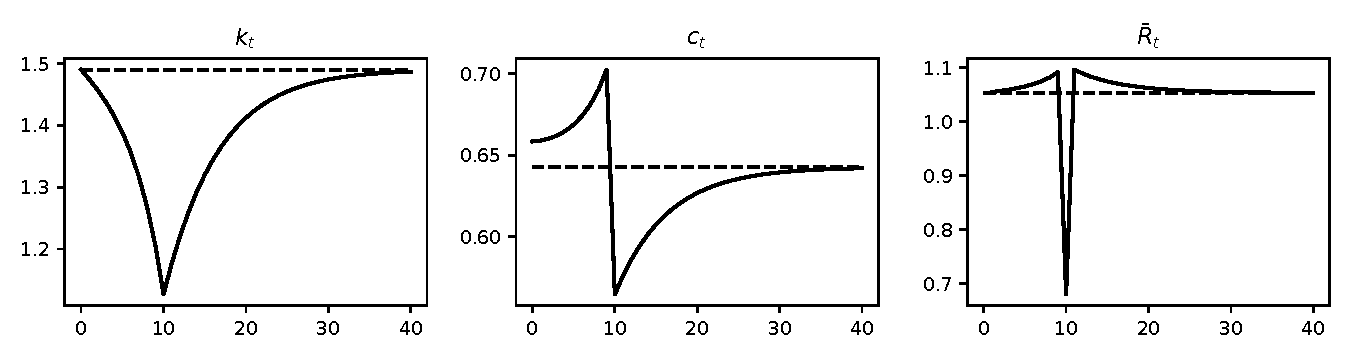
\includegraphics[width=.9\textwidth]{fig/ls11_01_tau_c.pdf}
\captionof{figure}{Exercise 11.1(e): consumption tax postponed to $t=10$ (solid) vs constant tax from $t=0$ (dashed).}
\end{center}
\end{tcolorbox}

%------- 11.2 -------
\begin{tcolorbox}[evenbox,title={Exercise 11.2 \quad Tax reform: II}]
\begin{longquestion}
p.~451. Consider the following economy populated by a government and a representative household. There is no
uncertainty, and the economy and the representative household and government within it last forever. The government
consumes a constant amount $g_t=g>0$, $t\ge0$. The government also sets sequences of two types of taxes,
$\{\tau_{ct},\tau_{kt}\}_{t=0}^\infty$. Here $\tau_{ct},\tau_{kt}$ are, respectively, a possibly time-varying flat-rate tax
on consumption and a time-varying flat-rate tax on earnings from capital. The preferences of the household are ordered by
$\sum_{t=0}^\infty\beta^tu(c_t)$, where $\beta\in(0,1)$ and $u(\cdot)$ is strictly concave, increasing, and twice
continuously differentiable. The household is endowed with one unit of labor each period and does not value leisure. The
feasibility condition in the economy is $g_t+c_t+k_{t+1}\le f(k_t)+(1-\delta)k_t$ where $k_t$ is the stock of capital
owned by the household at the beginning of time $t$ and $\delta\in(0,1)$ is a depreciation rate. At time 0, there are
complete markets for commodities at all dates. The household faces the budget constraint:
\[
\sum_{t=0}^\infty\{q_t[(1+\tau_{ct})c_t+k_{t+1}-(1-\delta)k_t]\}\le\sum_{t=0}^\infty q_t\{\eta_tk_t-\tau_{kt}(\eta_t-\delta)k_t+w_t\}
\]
where we assume that the household inelastically supplies one unit of labor, and $q_t$ is the price of date $t$
consumption goods in units of the numeraire at time 0, $\eta_t$ is the rental rate of date $t$ capital in units of time
$t$ goods, and $w_t$ is the wage rate of date $t$ labor in units of time $t$ goods.

A production firm rents labor and capital. The value of the firm is $\sum_{t=0}^\infty q_t[f(k_t)n_t-w_tn_t-\eta_tk_tn_t]$,
where here $k_t$ is the firm's capital-labor ratio and $n_t$ is the amount of labor it hires. The government sets
$\{g_t\}$ exogenously and must set the sequences $\{\tau_{ct},\tau_{kt}\}$ to satisfy the budget constraint:
\[
(1)\qquad\sum_{t=0}^\infty q_t\big(\tau_{ct}c_t+\tau_{kt}(\eta_t-\delta)k_t\big)=\sum_{t=0}^\infty q_tg_t.
\]

\textbf{a.} Define a competitive equilibrium.

\textbf{b.} Assume an initial situation in which from time $t\ge0$ onward, the government finances a constant stream of
expenditures $g_t=\bar g$ entirely by levying a constant tax rate $\tau_k$ on capital and a zero consumption tax. Tell how
to find steady-state levels of capital, consumption, and the rate of return on capital.

\textbf{c.} Let $\bar k_0$ be the steady value of $k_t$ that you found in part \textbf{b}. Let this be the initial value of
capital at time $t=0$ and consider the following experiment. Suddenly and unexpectedly, a new party comes into power that
repeals the tax on capital, sets $\tau_k=0$ forever, and finances the same constant level of $\bar g$ with a flat-rate tax
on consumption. Tell what happens to the new steady-state values of capital, consumption, and the return on capital.

\textbf{d.} Someone recommends comparing the two alternative policies of (1) relying completely on the taxation of capital
as in the initial equilibrium and (2) relying completely on the consumption tax, as in our second equilibrium, by
comparing the discounted utilities of consumption in steady state, i.e., by comparing $\frac1{1-\beta}u(\bar c)$ in the
two equilibria, where $\bar c$ is the steady-state value of consumption. Is this a good way to measure the costs or gains
of one policy \emph{vis-a-vis} the other?
\end{longquestion}

\textbf{Solution:}

\textbf{(a)} As in 11.1(a), with the policy $\{g_t,\tau_{ct},\tau_{kt}\}$ satisfying (1). The coefficient of $k_{t+1}$ in the
household budget is now $-q_t+q_{t+1}[(1-\tau_{k,t+1})(\eta_{t+1}-\delta)+1]$, so no arbitrage (11.5.2) gives
$q_t/q_{t+1}=(1-\tau_{k,t+1})(\eta_{t+1}-\delta)+1$. With $\beta^tu'(c_t)=\mu q_t(1+\tau_{ct})$ and $\eta=f'$, $w=f-kf'$, the
equilibrium solves (11.6.3) and (11.6.1), $k_0$ given, and the terminal condition (11.5.3).

\textbf{(b)} In a steady state (11.6.3) gives $1=\beta[(1-\tau_k)(f'(\kb)-\delta)+1]$, i.e.
\[
f'(\kb)=\delta+\frac{\rho}{1-\tau_k}\quad(11.6.7),\qquad \cb=f(\kb)-\delta\kb-\gb .
\]
Government budget: with everything constant, $q_t=\beta^tq_0$ and (1) becomes
$\tau_k(f'(\kb)-\delta)\kb\sum_tq_t=\gb\sum_tq_t$. Using (11.6.7), $(f'(\kb)-\delta)=\rho/(1-\tau_k)$, so the two unknowns
$(\kb,\tau_k)$ solve
\[
\kb=\kb(\tau_k)\equiv f'^{-1}\!\Big(\delta+\frac{\rho}{1-\tau_k}\Big),\qquad
\mathcal R(\tau_k)\equiv\frac{\tau_k\,\rho\,\kb(\tau_k)}{1-\tau_k}=\gb .
\]
$\mathcal R$ is a Laffer curve: zero at $\tau_k=0$, rising, then falling as $\kb(\tau_k)\to0$. Take the smallest root.
Returns: the after-tax gross return is $\Rb=1+\rho$ (11.6.10) whatever $\tau_k$; the pre-tax gross return
$f'(\kb)+1-\delta=1+\rho/(1-\tau_k)$ exceeds it.

\emph{Numbers.} With $f=k^{.33}$ the peak revenue is $\max\mathcal R=.146$ (at $\tau_k\approx.91$) $<.2$: the benchmark
$g=.2$ cannot be financed by a capital tax alone. We use $\gb=.05$: $\tau_k=.445443$, $\kb_0=1.182709$, $\cb=.770397$,
pre-tax $f'+1-\delta=1.094907$, $\Rb=1.052632$.

\textbf{(c)} With $\tau_k=0$ and a constant $\tau_c$, the tax ratio cancels from (11.6.3), so the equilibrium is the
planner's path from $\kb_0$ with $g_t=\gb$. New steady state: $f'(k^\ast)=\rho+\delta$. Since
$\rho+\delta<\delta+\rho/(1-\tau_k)$ and $f'$ is decreasing, $k^\ast>\kb_0$. Consumption
$c^\ast=f(k^\ast)-\delta k^\ast-\gb>\cb$ because $f(k)-\delta k$ is increasing for $k$ below the golden rule
$f'(k)=\delta$, and $k^\ast$ is below it. The after-tax return in steady state is $1+\rho$ in both regimes; the pre-tax
return falls from $1+\rho/(1-\tau_k)$ to $1+\rho$. Along the transition $k$ rises monotonically, $\Rb_{t}>1+\rho$ falls, and
$c$ rises; to build capital, consumption first falls below its old level. The constant tax is
$\tau_c=\gb\sum_tq_t/\sum_tq_tc_t$, computed on the transition path.

\emph{Numbers.} $k^\ast=1.489956$, $c^\ast=.792645$, pre-tax return $1.052632$; $c_0=.721969<\cb=.770397$;
$\tau_c=.064569$ (above the steady-state ratio $\gb/c^\ast=.063080$, because early consumption is low).

\textbf{(d)} No. Comparing $u(\cb)/(1-\beta)$ in the two steady states ignores that the economy starts at $\kb_0$, not at
$k^\ast$. To reach $k^\ast$ the household must first cut consumption and invest. The right comparison is
$\sum_t\beta^tu(c_t)$ along the equilibrium path from $\kb_0$ (part c) against $u(\cb_0)/(1-\beta)$. The steady-state
comparison overstates the gain from the reform. The gain is still positive: the path of (c) is the planner's optimum
from $\kb_0$, and staying at $(\kb_0,\cb_0)$ is feasible, so the reform cannot lower welfare.

\begin{tcolorbox}[databox]
$\gb=.05$. Consumption-equivalent gain of the reform: $2.888\%$ comparing steady states, $0.595\%$ including the
transition. Newton and shooting agree to $10^{-8}$. Figure: transition (left, centre) and the steady-state Laffer curve
$\mathcal R(\tau_k)$ with the level $\gb$ (right).
\end{tcolorbox}

\begin{center}
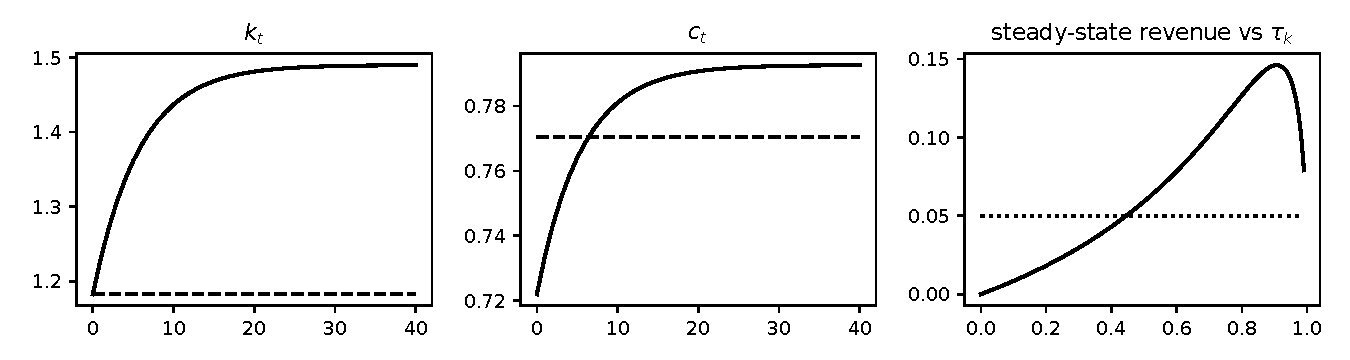
\includegraphics[width=.9\textwidth]{fig/ls11_02_tax_reform.pdf}
\captionof{figure}{Exercise 11.2: transition after the capital-tax repeal (dashed: initial steady state).}
\end{center}
\end{tcolorbox}

%------- 11.3 -------
\begin{tcolorbox}[oddbox,title={Exercise 11.3 \quad Anticipated productivity shift}]
\begin{tcolorbox}[questionbox]
p.~453. An infinitely lived representative household has preferences over a stream of consumption of a single good that
are ordered by $\sum_{t=0}^\infty\beta^tu(c_t)$, $\beta\in(0,1)$, where $u$ is a strictly concave, twice continuously
differentiable, one-period utility function, $\beta$ is a discount factor, and $c_t$ is time $t$ consumption. The
technology is:
\[
c_t+x_t\le f(k_t)n_t,\qquad k_{t+1}=(1-\delta)k_t+\psi_tx_t
\]
where for $t\ge1$, $\psi_t=1$ for $t<4$ and $\psi_t=2$ for $t\ge4$. Here $f(k_t)n_t$ is output, where $f>0$, $f'>0$,
$f''<0$, $k_t$ is capital per unit of labor input, and $n_t$ is labor input. The household supplies one unit of labor
inelastically. The initial capital stock $k_0$ is given and is owned by the representative household. In particular,
assume that $k_0$ is at the optimal steady value for $k$ presuming that $\psi_t$ had been equal to 1 forever. There is no
uncertainty. There is no government.

\textbf{a.} Formulate the planning problem for this economy in the space of sequences and form the pertinent Lagrangian.
Find a formula for the optimal steady-state level of capital. How does a permanent increase in $\psi$ affect the steady
values of $k$, $c$, and $x$?

\textbf{b.} Formulate the planning problem for this economy recursively (i.e., compose a Bellman equation for the
planner). Be careful to give a complete description of the state vector and its law of motion. (``Finding the state is
an art.'')

\textbf{c.} Formulate an (Arrow-Debreu) competitive equilibrium with time 0 trades, assuming the following
decentralization. Let the household own the stocks of capital and labor and in each period let the household rent them to
the firm. Let the household choose the investment rate each period. Define an appropriate price system and compute the
first-order necessary conditions for the household and for the firm.

\textbf{d.} What is the connection between a solution of the planning problem and the competitive equilibrium in part
c? Please link the prices in part c to corresponding objects in the planning problem.

\textbf{e.} Assume that $k_0$ is given by the steady-state value that corresponds to the assumption that $\psi_t$ had been
equal to 1 forever, and had been expected to remain equal to 1 forever. Qualitatively describe the evolution of the
economy from time 0 on. Does the jump in $\psi$ at $t=4$ have any effects that precede it?
\end{tcolorbox}

\textbf{Solution:} The statement defines $\psi_t$ for $t\ge1$; we take $\psi_0=1$. We do not impose $x_t\ge0$ (it never
binds in the computed path).

\textbf{(a)} With $n_t=1$, eliminate $x_t=[k_{t+1}-(1-\delta)k_t]/\psi_t$:
\[
\max\sum_t\beta^tu(c_t)\quad\text{s.t.}\quad c_t+\frac{k_{t+1}-(1-\delta)k_t}{\psi_t}\le f(k_t),\ k_0\text{ given};
\]
\[
\mathcal L=\sum_{t=0}^\infty\beta^t\Big\{u(c_t)+\mu_t\Big[f(k_t)-c_t-\frac{k_{t+1}-(1-\delta)k_t}{\psi_t}\Big]\Big\}.
\]
FOCs: $c_t$: $u'(c_t)=\mu_t$. $k_{t+1}$: $-\mu_t/\psi_t+\beta\mu_{t+1}[f'(k_{t+1})+(1-\delta)/\psi_{t+1}]=0$. Hence
\[
\frac{u'(c_t)}{\psi_t}=\beta u'(c_{t+1})\Big[f'(k_{t+1})+\frac{1-\delta}{\psi_{t+1}}\Big],\qquad
\lim_{t\to\infty}\beta^t\frac{u'(c_t)}{\psi_t}k_{t+1}=0 .\tag{11.3.1}
\]
Steady state with constant $\psi$: $1/\psi=\beta[f'(\kb)+(1-\delta)/\psi]$, so $1=\beta\psi f'(\kb)+\beta(1-\delta)$ and
\[
f'(\kb)=\frac{\rho+\delta}{\psi},\qquad \bar x=\frac{\delta\kb}{\psi},\qquad \cb=f(\kb)-\frac{\delta\kb}{\psi}.
\]
Comparative statics. $d\kb/d\psi=-f'(\kb)/(\psi f''(\kb))>0$.
$d\cb/d\psi=[f'(\kb)-\delta/\psi]\,d\kb/d\psi+\delta\kb/\psi^2=(\rho/\psi)\,d\kb/d\psi+\delta\kb/\psi^2>0$.
With the elasticity $\varepsilon\equiv(\psi/\kb)d\kb/d\psi=-f'/(\kb f'')$,
$d\bar x/d\psi=(\delta/\psi)d\kb/d\psi-\delta\kb/\psi^2=(\delta\kb/\psi^2)(\varepsilon-1)$: investment in goods rises iff
$\varepsilon>1$. For $f=zk^\alpha$, $\kb\propto\psi^{1/(1-\alpha)}$ and $\varepsilon=1/(1-\alpha)>1$, so $x$ rises. So
a permanent rise in $\psi$ raises $k$, $c$ and (Cobb--Douglas) $x$.

\textbf{(b)} The problem is not stationary in $t$, but the only relevant information about the future is how far the
economy is from the shift. State: $(k_t,s_t)$ with $s_t=\min\{t,4\}$, law of motion $s_{t+1}=\min\{s_t+1,4\}$, and
$\psi(s)=1$ for $s<4$, $\psi(4)=2$ (so $\psi_t=\psi(s_t)$). Bellman equation:
\[
V(k,s)=\max_{k'}\Big\{u\Big(f(k)-\frac{k'-(1-\delta)k}{\psi(s)}\Big)+\beta V\big(k',\min\{s+1,4\}\big)\Big\}.
\]
$V(\cdot,4)$ is the stationary value function with $\psi=2$ (a fixed point); $V(\cdot,3),\dots,V(\cdot,0)$ follow by four
backward Bellman steps. FOC $u'(c)/\psi(s)=\beta V_k(k',s')$ and envelope
$V_k(k,s)=u'(c)[f'(k)+(1-\delta)/\psi(s)]$ give (11.3.1).

\textbf{(c)} Price system $\{q_t,\eta_t,w_t\}$: $q_t$ is the time-0 price of a unit of the time-$t$ good (consumption and
investment are the same good), $\eta_t$ the rental rate of capital and $w_t$ the wage, both in time-$t$ goods. Household:
\[
\max\sum_t\beta^tu(c_t)\ \text{ s.t. }\ \sum_tq_t(c_t+x_t)\le\sum_tq_t(\eta_tk_t+w_t),\quad k_{t+1}=(1-\delta)k_t+\psi_tx_t .
\]
Substituting $x_t$, the coefficient of $k_{t+1}$ in the budget is $-q_t/\psi_t+q_{t+1}[\eta_{t+1}+(1-\delta)/\psi_{t+1}]$.
FOCs:
\[
\beta^tu'(c_t)=\mu q_t,\qquad \frac{q_t}{\psi_t}=q_{t+1}\Big[\eta_{t+1}+\frac{1-\delta}{\psi_{t+1}}\Big].
\]
The price of a unit of installed capital is $q_t/\psi_t$ (i.e.\ $1/\psi_t$ goods). Firm: $\max\sum_tq_t[f(k_t)n_t-w_tn_t-\eta_tk_tn_t]$
gives $\eta_t=f'(k_t)$, $w_t=f(k_t)-k_tf'(k_t)$.

\textbf{(d)} Substituting the firm's conditions and $q_t=\beta^tu'(c_t)/\mu$ into the household's conditions gives exactly
(11.3.1) and feasibility: the competitive allocation solves the planning problem and conversely (welfare theorems). The
prices are the planner's multipliers: $q_t=\beta^t\mu_t/\mu$ (resource constraint, discounted), $q_t/\psi_t$ the shadow
value of installed capital, $\eta_t=f'(k_t)$ its marginal product, $w_t$ the marginal product of labour.

\textbf{(e)} Yes, the shift has effects before $t=4$. Two forces act from $t=0$:
\begin{itemize}[itemsep=2pt]
\item \emph{Wealth.} Future output will be higher, so the household wants to consume more now.
\item \emph{Capital loss.} Capital bought at $t=3$ costs one good per unit, but at $t=4$ new capital costs only $1/2$ a
good. By (11.3.1), the gross return from $3$ to $4$ is $\psi_3[f'(k_4)+(1-\delta)/\psi_4]=f'(k_4)+(1-\delta)/2$: the
undepreciated capital loses half its value. Saving into $t=4$ is unattractive.
\end{itemize}
So between $t=0$ and $3$ consumption rises and investment falls, and $k$ declines. The low return from $3$ to $4$ implies
$c_4<c_3$ by (11.3.1). At $t=4$ investment becomes twice as productive, investment surges, and $k$ and $c$ rise toward the
new steady state, with high returns along the way.

\begin{tcolorbox}[databox]
$g=0$, $\psi_0=1$. Steady states: $\psi=1$: $(k,x,c)=(1.489956,.297991,.842645)$; $\psi=2$:
$(4.192491,.419249,1.185532)$, with $k$ multiplied by $2^{1/(1-\alpha)}$.

\smallskip
\resizebox{\linewidth}{!}{%
\begin{tabular}{@{}lcccccccc@{}}
\toprule
$t$ & 0 & 1 & 2 & 3 & 4 & 5 & 6 & 7\\
\midrule
$k_t$ & 1.4900 & 1.4317 & 1.3672 & 1.2922 & 1.2009 & 1.5916 & 1.9555 & 2.2835\\
$c_t$ & .9009 & .9039 & .9103 & .9211 & .7468 & .8246 & .8882 & .9402\\
$x_t$ & .2397 & .2218 & .1984 & .1671 & .3154 & .3411 & .3595 & .3730\\
return $t\to t+1$ & 1.0595 & 1.0676 & 1.0779 & .6919 & 1.2834 & 1.2211 & 1.1796 & 1.1504\\
\bottomrule
\end{tabular}}

\smallskip
Newton and shooting agree to $10^{-8}$; $x_t>0$ throughout.
\end{tcolorbox}

\begin{center}
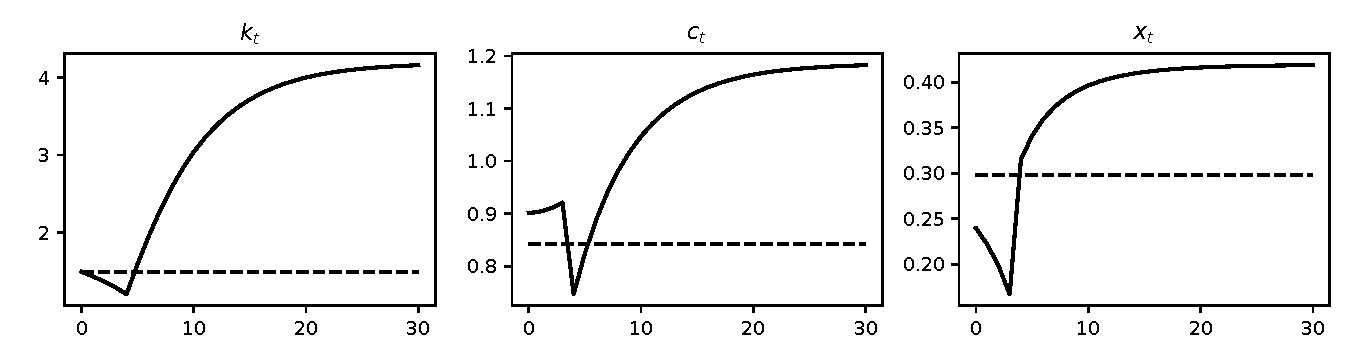
\includegraphics[width=.9\textwidth]{fig/ls11_03_psi.pdf}
\captionof{figure}{Exercise 11.3: responses to the shift in $\psi$ at $t=4$, known at $t=0$ (dashed: old steady state).}
\end{center}
\end{tcolorbox}

%------- 11.4 -------
\begin{tcolorbox}[evenbox,title={Exercise 11.4 \quad A capital levy}]
\begin{longquestion}
p.~454. A nonstochastic economy produces one good that can be allocated among consumption, $c_t$, government purchases,
$g_t$, and gross investment, $x_t$. The economy-wide resource constraints are
\[
c_t+g_t+x_t\le f(k_t),\qquad k_{t+1}=(1-\delta)k_t+x_t,
\]
where $\delta\in(0,1)$ is a depreciation rate, $k_t$ is the capital stock, and $f(k_t)$ gives production as a function of
capital, where $f(k)=Ak^\alpha$ with $\alpha\in(0,1)$. A single representative consumer owns the capital stock and one
unit of labor. The consumer rents capital and labor to a competitive firm each period. The consumer ranks consumption
plans according to $\sum_{t=0}^\infty\beta^tu(c_t)$ where $u(c)=\frac{c^{1-\gamma}}{1-\gamma}$, with $\gamma\ge1$. The
household supplies one unit of labor inelastically each period.

The government has only one tax at its disposal, a one-time capital levy through which it confiscates part of the capital
stock from the private sector. When the government imposes a capital levy, we assume that it sends the consumer a tax bill
for a fraction $\phi$ of the beginning of period capital stock. Below, you will be asked to compare consequences of
levying this tax either at the beginning of time $T=0$ or at the beginning of time $T=10$. The fraction can exceed 1 if
that is necessary to finance the government budget. The government is allowed to impose no other taxes. Among other
things, this means that it cannot impose a direct lump sum or `head' tax.

\textbf{a.} Define a competitive equilibrium with time 0 trading.

\textbf{b.} Suppose that before time 0 the economy had been in a steady state in which $g$ had always been zero and had
been expected always to equal zero. Find a formula for the initial steady state capital stock in a competitive
equilibrium with time zero trading. Let this value be $\bar k_0$.

\textbf{c.} At time 0, everyone suddenly wakes up to discover that from time 0 on, government expenditures will be
$\bar g>0$, where $\bar g+\delta\bar k_0<f(\bar k_0)$, which implies that the new level of government expenditures would
be feasible in the old steady state. Suppose that the government finances the new path of expenditures by a capital levy
at time $T=0$. The government imposes a capital levy by sending the household a bill for a fraction of the value of its
capital at the time indicated. Find the new steady state value of the capital stock in a competitive equilibrium.
Describe an algorithm to compute the fraction of the capital stock that the government must tax away at time 0 to
finance its budget. Find the new steady state value of the capital stock in a competitive equilibrium. Describe the time
paths of capital, consumption, and the interest rate from $t=0$ to $t=+\infty$ in the new equilibrium and compare them
with their counterparts in the initial $g_t\equiv0$ equilibrium.

\textbf{d.} Assume the same new path of government expenditures indicated in part \textbf{c}, but now assume that the
government imposes the one-time capital levy at time $T=10$, and that this is foreseen at time 0. Find the new steady
state value of the capital stock in a competitive equilibrium that is associated with this tax policy. Describe an
algorithm to compute the fraction of the capital stock that the government must tax away at time $T=10$ to finance its
budget. Describe the time paths of capital, consumption, and the interest rate in this new equilibrium and compare them
with their counterparts in part \textbf{b} and in the initial $g_t\equiv0$ equilibrium.

\textbf{e.} Define a competitive equilibrium with sequential trading of one-period Arrow securities. Describe how to
compute such an equilibrium. Describe the time path of the consumer's holdings of one-period securities in a competitive
equilibrium with one period Arrow securities under the government tax policy assumed in part \textbf{d}. Describe the
time path of government debt.
\end{longquestion}

\textbf{Solution:} \emph{Reading.} The bill is $\phi k_T$ units of time-$T$ goods; the household keeps its capital and
its rentals. (Confiscating $\phi k_T$ physical units is the same thing, since capital and goods convert one-for-one.)
Parts (d) and (e) compare with ``part b'', which we read as the initial $g\equiv0$ steady state.

\textbf{(a)} A competitive equilibrium is prices $\{q_t,\eta_t,w_t\}$, a policy $(\{g_t\},\phi,T)$, and an allocation
$\{c_t,x_t,k_{t+1}\}$ such that: the household maximises $\sum_t\beta^tu(c_t)$ subject to
\[
\sum_tq_t(c_t+x_t)\le\sum_tq_t(\eta_tk_t+w_t)-q_T\phi k_T,\qquad k_{t+1}=(1-\delta)k_t+x_t,\ k_0\text{ given};
\]
the firm sets $\eta_t=f'(k_t)=\alpha Ak_t^{\alpha-1}$, $w_t=f(k_t)-k_tf'(k_t)$; the government budget holds,
$q_T\phi k_T=\sum_tq_tg_t$; and $c_t+g_t+x_t=f(k_t)$. Collecting terms in $k_{t+1}$ gives no-arbitrage conditions
$q_t=q_{t+1}[\eta_{t+1}+1-\delta]$ for $t+1\neq T$ and $q_{T-1}=q_T[\eta_T+1-\delta-\phi]$ if $T\ge1$. With
$\beta^tu'(c_t)=\mu q_t$:
\[
u'(c_t)=\beta u'(c_{t+1})\big[f'(k_{t+1})+1-\delta-\phi\,\mathbf 1\{t+1=T\}\big].\tag{11.4.1}
\]

\textbf{(b)} $g\equiv0$, steady state: $1=\beta[f'(\kb_0)+1-\delta]$, so
$\alpha A\kb_0^{\alpha-1}=\rho+\delta$ and $\kb_0=\big(\alpha A/(\rho+\delta)\big)^{1/(1-\alpha)}$;
$\cb_0=A\kb_0^\alpha-\delta\kb_0$.

\textbf{(c)} $T=0$: $k_0$ is given, so the bill $\phi k_0$ cannot be avoided and is a lump-sum tax; $\phi$ never enters
(11.4.1) (which involves $k_{t+1}$, $t+1\ge1$). The allocation is the planner's with $g_t=\gb$. New steady state: from
(11.4.1), $f'(\kb)=\rho+\delta$, so $\kb=\kb_0$ (the level of $g$ does not enter). Since $k_0=\kb_0$ is already the new
steady state, the equilibrium is
\[
k_t=\kb_0,\qquad c_t=\cb_0-\gb,\qquad q_t=\beta^t,\qquad R_{t,t+1}=1/\beta=1+\rho\ \text{ for all }t\ge0 .
\]
\emph{Algorithm} (general $k_0$ and $\{g_t\}$): (1) compute the planner's path by shooting on (11.4.1) with $\phi=0$;
(2) $q_t=\beta^tu'(c_t)/u'(c_0)$; (3) $\phi=\sum_tq_tg_t/(q_0k_0)$. Here $\phi=\gb/((1-\beta)\kb_0)$, which exceeds 1
when $\gb>(1-\beta)\kb_0$; the household pays out of its total wealth, including the present value of wages.
\emph{Comparison with $g\equiv0$}: same capital and interest rate; consumption lower by exactly $\gb$ at every date.

\textbf{(d)} $T=10$ foreseen. Now $k_{10}$ is chosen knowing the levy: by (11.4.1) the gross return on capital carried
from 9 to 10 is $f'(k_{10})+1-\delta-\phi$. The levy is a one-time tax on capital, a distorting tax. After $t=10$ nothing
distorts: the new steady state is again $\kb=\kb_0$.

\emph{Algorithm for $\phi$.} (1) Guess $\phi$. (2) Solve (11.4.1) and feasibility with $g_t=\gb$ by shooting from $\kb_0$
toward $\kb_0$. (3) Compute $q_t=\beta^tu'(c_t)/u'(c_0)$. (4) Evaluate the gap $G(\phi)=\phi q_{10}k_{10}-\gb\sum_tq_t$.
(5) Update $\phi$ by bisection on the rising side of the Laffer curve. A Laffer curve appears because a higher $\phi$ lowers
$k_{10}$: the Euler equation needs $f'(k_{10})\approx\rho+\delta+\phi$. So revenue $\phi q_{10}k_{10}$ has a maximum, and
an equilibrium exists only if that maximum covers $\gb\sum_tq_t$.

\emph{Paths.} Before 10, capital is run down (it will be taxed); consumption jumps above its $T=0$ level and rises
until $t=9$, because $\Rb_{t+1}=f'(k_{t+1})+1-\delta>1+\rho$ as $k$ falls. The interest rate from 9 to 10 is very low
(the return net of the levy). At 10 consumption drops. After 10 capital is rebuilt: the interest rate jumps above $\rho$ and
falls back, and consumption rises back to $\cb_0-\gb$. Compared with the initial $g\equiv0$ steady state: the long run is
the same except that $c$ is lower by $\gb$. Compared with $T=0$: the same long run, but a distorted transition and lower
welfare.

\begin{tcolorbox}[databox]
$A=1$, benchmark $\alpha,\beta,\delta,\gamma$: $\kb_0=1.489956$, $\cb_0=.842645$.
\emph{Existence at $T=10$:} the levy can finance $\gb$ only if $\gb\le.03541$. With the benchmark $\gb=.2$ the peak of the
Laffer curve ($\phi=5.80$) raises only $32\%$ of the present value of spending, so no equilibrium exists. We use
$\gb=.02$.

(c) $\phi=\gb/((1-\beta)\kb_0)=.268464$; $c_t=.822645$; $r=-\log\beta=.051293$.
(d) $\phi=.494143$ (peak of the Laffer curve at $\phi=1.516$); $k_{10}=1.012095$; $c_0=.840408$, $c_9=.911460$,
$c_{10}=.706924$; $r_{9,10}=-.456955$, $r_{10,11}=.106263$. Welfare $-24.3118$ ($T=0$) $>-24.4418$ ($T=10$).
Newton and shooting agree to $10^{-8}$.
\end{tcolorbox}

\textbf{(e)} With no uncertainty, one-period Arrow securities are one-period risk-free bonds. Let $b_t$ be the household's
claims on time-$t$ goods bought at $t-1$ at price $1/R_{t-1,t}$, $b_0=0$. Household at each $t$:
\[
c_t+k_{t+1}+\frac{b_{t+1}}{R_{t,t+1}}=\eta_tk_t+w_t+(1-\delta)k_t+b_t-\phi k_t\mathbf 1\{t=T\},
\]
with a natural debt limit on $b_{t+1}$. Government: $g_t+b_t=b_{t+1}/R_{t,t+1}+\phi k_t\mathbf 1\{t=T\}$. A sequential
equilibrium is prices $\{R_{t,t+1},\eta_t,w_t\}$ and quantities such that both budgets hold, the household and firm
optimise, and the goods and bond markets clear. \emph{Computation:} solve the time-0 equilibrium of (d); set
$R_{t,t+1}=q_t/q_{t+1}$; then the bond position is the government debt in (11.4.3),
\[
B_t\equiv\frac{b_{t+1}}{R_{t,t+1}}=\sum_{s>t}\frac{q_s}{q_t}(T_s-g_s),\qquad T_s=\phi k_{10}\mathbf 1\{s=10\}.
\]
\emph{Paths under (d).} For $t<10$ the government has no revenue and borrows: $B_t$ grows ($B_t=g_t+R_{t-1,t}B_{t-1}$), and
the household lends. At $t=10$ the levy exceeds the debt and the government becomes a creditor: $B_{10}<0$, i.e.\ the
household is now in debt to the government. From then on the household pays interest on that debt, and the interest
finances $\gb$. In the limit $\gb+R B=B$, so $B_\infty=-\gb/\rho$.

\begin{tcolorbox}[databox]
$\gb=.02$: $B_0=.02$, $B_9=.287525$, $B_{10}=-.298057$, $B_t\to-\gb/\rho=-.38$. The sequential budget (11.4.2)
$g_t+R_{t-1,t}B_{t-1}=T_t+B_t$ holds date by date (checked).
\end{tcolorbox}

\begin{center}
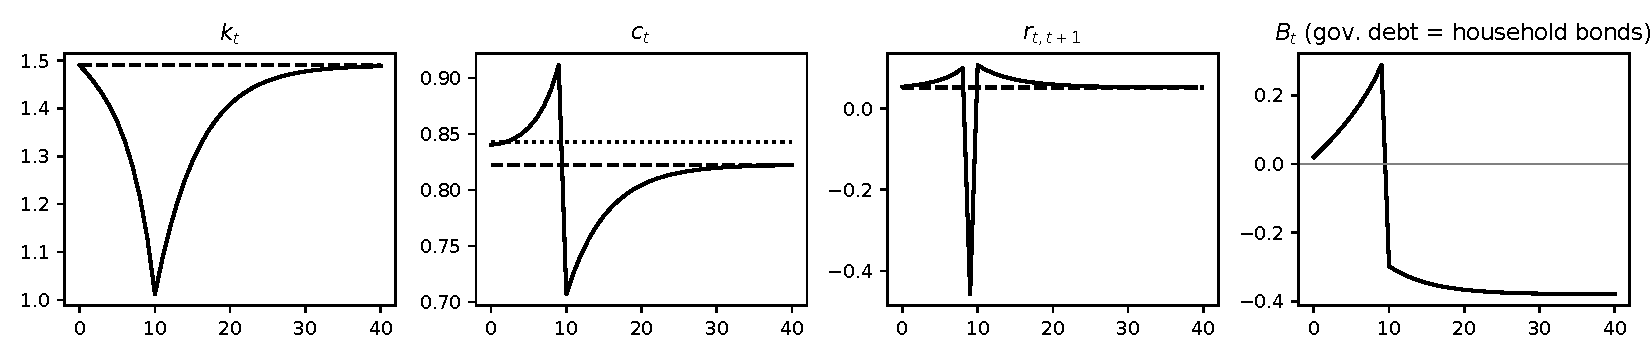
\includegraphics[width=\textwidth]{fig/ls11_04_levy.pdf}
\captionof{figure}{Exercise 11.4 ($\gb=.02$): levy at $T=10$ (solid) vs $T=0$ (dashed); dotted: $g\equiv0$ consumption.}
\end{center}
\end{tcolorbox}

%----------------------------------------------------------------------
\subsection{Steady States, Open Economies and Linear Utility (11.5--11.9)}
%----------------------------------------------------------------------

%------- 11.5 -------
\begin{tcolorbox}[oddbox,title={Exercise 11.5 \quad Log utility, the golden rule and a jump in $g$}]
\begin{tcolorbox}[questionbox]
p.~456. A representative consumer has preferences ordered by $\sum_{t=0}^\infty\beta^t\log(c_t)$, $0<\beta<1$, where
$\beta=\frac1{1+\rho}$, $\rho>0$, and $c_t$ is the consumption per worker. The technology is
\[
y_t=f(k_t)=zk_t^\alpha,\quad0<\alpha<1,\quad z>0
\]
where $y_t$ is the output per unit labor and $k_t$ is capital per unit labor
\[
y_t=c_t+x_t+g_t,\qquad k_{t+1}=(1-\delta)k_t+x_t,\quad0<\delta<1
\]
and $x_t$ is gross investment per unit of labor and $g_t$ is government expenditures per unit of labor. Assume a
competitive equilibrium with a price system $\{q_t,\eta_t,w_t\}_{t=0}^\infty$ and a government policy
$\{g_t,\tau_{ht}\}_{t=0}^\infty$.

Assume that the government finances its expenditures by levying lump sum taxes. There are no distorting taxes. Assume
that at time 0, the economy begins with a capital per unit of labor $k_0$ that equals the steady state value appropriate
for an economy in which $g_t$ had been zero forever.

\textbf{a.} Find a formula for the steady state capital stock when $g_t=0\ \forall t$.

\textbf{b.} Compare the steady state capital labor ratio $\bar k$ in the competitive equilibrium with the capital labor
ratio $\tilde k$ that maximizes steady state consumption per capita, i.e., $\tilde k$ solves
$\tilde c=\max_k\big(f(k)-\delta k\big)$. Is $\tilde k$ greater than or less that $\bar k$? If they differ, please tell
why. Is $\tilde c$ greater or less than $\bar c=f(\bar k)-\delta\bar k$? Explain why.

\textbf{c.} Now assume that at time 0, $g_t$ suddenly jumps to the value $g=\frac12\bar c$ where $\bar c$ is the value of
consumption per capita in the initial steady state in which $g$ was zero forever. Starting from $k_0=\bar k$ for the old
$g=0$ steady state, find the time paths of $\{c_t,k_{t+1}\}_{t=0}^\infty$ associated with the new path $g_t=g>0\ \forall t$
for government expenditures per capita. Also show the time path for $\bar R_{t+1}\equiv(1-\delta)+f'(k_{t+1})$. Explain
why the new paths are as they are.
\end{tcolorbox}

\textbf{Solution:} With lump-sum taxes the equilibrium is the planner's allocation with $g_t$ deducted from output
(section 11.8), and (11.6.3) with $u=\log$ reads $c_{t+1}/c_t=\beta[f'(k_{t+1})+1-\delta]$.

\textbf{(a)} Steady state: $1=\beta[f'(\kb)+1-\delta]$, i.e.\ $\alpha z\kb^{\alpha-1}=\rho+\delta$:
\[
\kb=\Big(\frac{\alpha z}{\rho+\delta}\Big)^{\frac1{1-\alpha}},\qquad \cb=z\kb^\alpha-\delta\kb .
\]

\textbf{(b)} $\tilde k$ maximises $f(k)-\delta k$: $f'(\tilde k)=\delta$, so $\tilde k=(\alpha z/\delta)^{1/(1-\alpha)}$.
Since $\rho+\delta>\delta$ and $f'$ is decreasing, $\tilde k>\kb$. And $\tilde c\ge\cb$ by definition of $\tilde k$,
strictly because $\kb\ne\tilde k$ and $f(k)-\delta k$ is strictly concave. Why they differ: the household discounts the
future. At $\kb$ the net marginal product $f'(\kb)-\delta=\rho$ just compensates for impatience. Moving from $\kb$ toward
$\tilde k$ would require giving up consumption now for a permanent gain later that yields less than $\rho$ per period, so
it is not worth it. $\kb$ is the ``modified'' (or augmented, section 11.6.2) golden rule.

\textbf{(c)} $g$ does not enter the steady-state Euler equation, so the new steady state is still $\kb$. Check that the
constant path
\[
k_t=\kb,\qquad c_t=f(\kb)-\delta\kb-g=\cb-g=\tfrac12\cb,\qquad \Rb_{t+1}=f'(\kb)+1-\delta=1+\rho\quad\forall t\ge0
\]
is the equilibrium: feasibility holds; $c_{t+1}/c_t=1=\beta(1+\rho)$ is the Euler equation; the terminal condition holds.
The solution of the (concave) planning problem is unique, so this is the only equilibrium. Explanation: a permanent,
unforeseen rise in $g$ financed by lump-sum taxes is a pure wealth effect. The household's present value of taxes rises by
$g\sum_tq_t$; it smooths the loss by cutting consumption by $g$ at every date. The return on capital is unchanged, so there
is no reason to change the capital stock. Government purchases crowd out consumption one-for-one and investment not at all.

\begin{tcolorbox}[databox]
$z=1$, benchmark $\alpha,\beta,\delta$: $\kb=1.489956$, $\cb=.842645$; $\tilde k=2.111557$, $\tilde c=.857420$.
(c) $g=.421323$: the Newton path is $k_t=1.489956$, $c_t=.421323$, $\Rb_{t+1}=1.052632$ for all $t$ (checked).
\end{tcolorbox}
\end{tcolorbox}

%------- 11.6 -------
\begin{tcolorbox}[evenbox,title={Exercise 11.6 \quad Trade and growth}]
\begin{tcolorbox}[questionbox]
p.~457. \textbf{Part I.} Consider the problem of a planner in a small economy. When the economy is closed to
international trade, the planner chooses $\{c_t,k_{t+1}\}_{t=0}^\infty$ to maximize $\sum_{t=0}^\infty\beta^tu(c_t)$, where
$0<\beta<1$, $\beta=\frac1{1+\rho}$, $\rho>0$ subject to
\[
c_t+k_{t+1}=f(k_t)+(1-\delta)k_t,\quad\delta\in(0,1)
\]
where $u(c_t)=\frac{c_t^{1-\gamma}}{1-\gamma}$, $\gamma>0$, $f(k_t)=zk_t^\alpha$, and $0<\alpha<1$. Let $\bar k$ be the
steady state value of $k_t$ under the optimal plan.

\textbf{a.} Find a formula for $\bar k$.

\textbf{b.} Assume that $k_0<\bar k$. Describe time paths for $\{c_t,k_{t+1}\}_{t=0}^\infty$ and
$\bar R_{t+1}=(1-\delta)+f'(k_{t+1})$.

\textbf{c.} What is the steady state value of $\bar R_{t+1}$?

\textbf{d.} Is $\bar R_{t+1}$ less or greater than its steady state value when $k_{t+1}<\bar k$?

\textbf{Part II.} Now assume that the economy is open to international trade in capital and financial assets. Assume that
there is a fixed world gross rate of return $R=\beta^{-1}$ at which the planner can borrow or lend, what is often called a
`small open economy' assumption. The planner can use the proceeds of borrowing to purchase goods on the international
market. These goods can be used to augment capital or to consume.

Let $\bar k_0$ be the level of initial capital ($\bar k_0<\bar k$) before the country opens up to trade just before time
0. Let $\bar k_0$ be the same initial capital per capita $\bar k_0<\bar k$ studied in parts \textbf{a-d}.

At time $t=-1$, after $\bar k_0$ was set, trade opens up. At time $t=-1$, the planner can issue IOU's or bonds in amount
$B_{-1}$ and use the proceeds to purchase capital, thereby setting $k_0=\bar k_0+B_{-1}$ where $B_{-1}$ is denominated in
time -1 consumption goods. The bonds are one period in duration and bear the constant world gross interest rate
$R=\beta^{-1}$. For $t\ge0$, the planner faces the constraints
\[
c_t+k_{t+1}+RB_{t-1}=f(k_t)+(1-\delta)k_t+B_t
\]
Here $RB_{t-1}$ is the sum of interest and principal on the bonds issued at $t-1$ and $B_t$ is the amount of one-period
bonds issued at $t$.

The planning problem in the small open economy is now to choose $\{c_t,k_t,B_t\}_{t=0}^\infty$ and $B_{-1}$, subject to
$\bar k_0$ given. (Notice that $k_0$ is a choice variable and that $\bar k_0$ is an initial condition.) Please solve the
planning problem in the small open economy and compare outcomes to those in the closed economy. Is welfare
$\sum_{t=0}^\infty\beta^tu(c_t)$ higher in the ``open'' or ``closed'' economy?
\end{tcolorbox}

\textbf{Solution:}

\textbf{Part I. (a)} Lagrangian $\sum_t\beta^t\{u(c_t)+\mu_t[f(k_t)+(1-\delta)k_t-c_t-k_{t+1}]\}$; FOCs $u'(c_t)=\mu_t$ and
$\mu_t=\beta\mu_{t+1}[f'(k_{t+1})+1-\delta]$, so $c_t^{-\gamma}=\beta c_{t+1}^{-\gamma}\Rb_{t+1}$. Steady state
$\beta\Rb=1$:
\[
\alpha z\kb^{\alpha-1}=\rho+\delta\quad\Rightarrow\quad\kb=\Big(\frac{\alpha z}{\rho+\delta}\Big)^{\frac1{1-\alpha}}.
\]

\textbf{(b)} With $k_0<\kb$, the optimal policy $k_{t+1}=h(k_t)$ is increasing with $h(k)>k$ for $k<\kb$, so $k_t$ rises
monotonically to $\kb$. Along the path $k_{t+1}<\kb$, so $f'(k_{t+1})>\rho+\delta$ and $\Rb_{t+1}>1+\rho$; then by the
Euler equation $c_{t+1}/c_t=(\beta\Rb_{t+1})^{1/\gamma}>1$: consumption rises monotonically to
$\cb=f(\kb)-\delta\kb$. $\Rb_{t+1}$ falls monotonically to $1+\rho$ as $k_{t+1}$ rises.

\textbf{(c)} $\Rb=f'(\kb)+1-\delta=1+\rho=\beta^{-1}$.

\textbf{(d)} Greater: $f'$ is decreasing, so $k_{t+1}<\kb$ implies $f'(k_{t+1})>f'(\kb)$ and $\Rb_{t+1}>1+\rho$.

\textbf{Part II.} Lagrangian with multipliers $\beta^t\mu_t$ on the period-$t$ constraints ($t\ge0$), using
$k_0=\kb_0+B_{-1}$:
\[
\mathcal L=\sum_{t\ge0}\beta^t\big\{u(c_t)+\mu_t[f(k_t)+(1-\delta)k_t+B_t-c_t-k_{t+1}-RB_{t-1}]\big\}.
\]
FOCs:
\begin{itemize}[itemsep=2pt]
\item $c_t$: $u'(c_t)=\mu_t$.
\item $B_t$ ($t\ge0$): $\beta^t\mu_t-\beta^{t+1}R\mu_{t+1}=0$, so $u'(c_t)=\beta Ru'(c_{t+1})=u'(c_{t+1})$: \emph{constant
consumption}.
\item $k_{t+1}$ ($t\ge0$): $\mu_t=\beta\mu_{t+1}[f'(k_{t+1})+1-\delta]$, so $f'(k_{t+1})+1-\delta=R=1+\rho$: $k_{t+1}=\kb$.
\item $B_{-1}$ (enters through $k_0=\kb_0+B_{-1}$ and the repayment $RB_{-1}$): $\mu_0[f'(k_0)+1-\delta-R]=0$, so
$k_0=\kb$ and $B_{-1}=\kb-\kb_0>0$: the country borrows abroad to install the steady-state capital at once.
\end{itemize}
Consumption level. Multiply the constraint at $t$ by $R^{-t}=\beta^t$ and sum; with $k_t=\kb$ and the no-Ponzi condition
$\lim_TR^{-T}B_T=0$ the $B$ terms telescope to $-RB_{-1}$:
\[
\sum_t\beta^tc_t=\frac{f(\kb)-\delta\kb}{1-\beta}-RB_{-1}\ \Rightarrow\
\boxed{c=f(\kb)-\delta\kb-\frac{1-\beta}{\beta}B_{-1}=f(\kb)-\delta\kb-\rho(\kb-\kb_0).}
\]
Debt. From the constraint, $B_t-RB_{t-1}=c-f(\kb)+\delta\kb=-\rho B_{-1}$. At $t=0$, $B_0=(R-\rho)B_{-1}=B_{-1}$; by
induction $B_t=B_{-1}$ for all $t$: the country rolls over its debt and pays interest $\rho B_{-1}$ each period.

Comparison. The open economy jumps immediately to $\kb$ and has flat consumption and $\Rb=1+\rho$ throughout. The closed
economy approaches $\kb$ gradually, with rising consumption and $\Rb>1+\rho$. Welfare is higher in the open economy. The
closed-economy plan ($B_t=0$ for all $t$, $k_0=\kb_0$) is feasible in the open economy, so the open optimum is at least as
good. It is strictly better because the closed plan has rising consumption, which violates the open economy's FOC
$u'(c_t)=u'(c_{t+1})$.

\begin{tcolorbox}[databox]
$z=1$, $g=0$, $\kb_0=.5\kb$. Closed: $k_0=.744978\to1.489956$, $c_0=.647540\to.842645$, $\Rb_1=1.166272\to1.052632$
(monotone paths checked). Open: $B_{-1}=.744978$, $c=.803436$, interest $\rho B_{-1}=.039209$ per period; PV and period
budgets checked. Welfare $-25.2394$ (closed) $<-24.8931$ (open): the open economy is worth $1.391\%$ more consumption
every period.
\end{tcolorbox}

\begin{center}
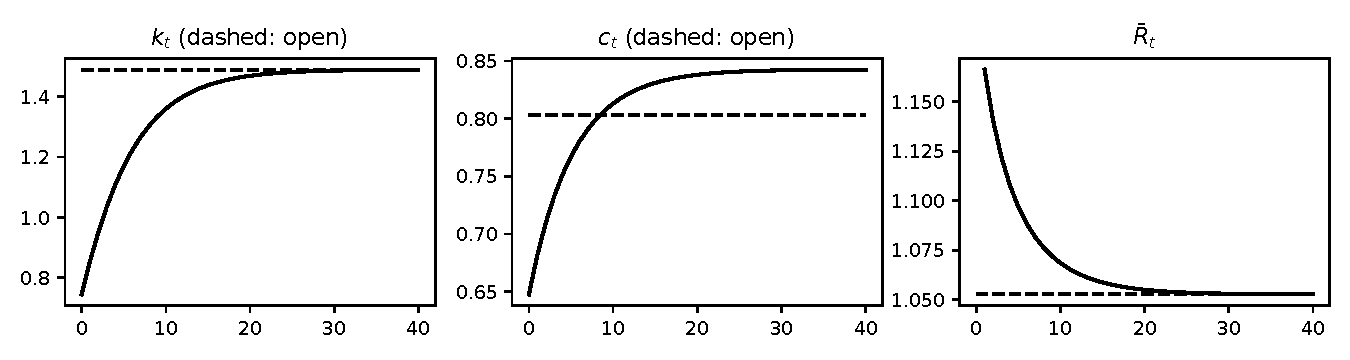
\includegraphics[width=.9\textwidth]{fig/ls11_06_open.pdf}
\captionof{figure}{Exercise 11.6: closed economy from $\kb_0=.5\kb$ (solid) and the small open economy (dashed).}
\end{center}
\end{tcolorbox}

%------- 11.7 -------
\begin{tcolorbox}[oddbox,title={Exercise 11.7 \quad Capital taxes: unforeseen, foreseen, and the role of $\gamma$}]
\begin{tcolorbox}[questionbox]
p.~458. The next several problems assume the following environment. A representative consumer has preferences ordered by
$\sum_{t=0}^\infty\beta^tu(c_t)$, $0<\beta<1$, $\beta=\frac1{1+\rho}$, $\rho>0$, where $c_t$ is the consumption per worker
and where $u(c)=\frac{c^{1-\gamma}}{1-\gamma}$ for $\gamma>0$ and $\gamma\ne1$, $u(c)=\log(c)$ if $\gamma=1$. The technology
is $y_t=f(k_t)=zk_t^\alpha$, $0<\alpha<1$, $z>0$, where $y_t$ is the output per unit labor and $k_t$ is capital per unit
labor and
\[
y_t=c_t+x_t+g_t,\qquad k_{t+1}=(1-\delta)k_t+x_t,\quad0<\delta<1
\]
where $x_t$ is gross investment per unit of labor and $g_t$ is government expenditures per unit of labor. The government
finances its expenditures by levying some combination of a flat rate tax $\tau_{ct}$ on the value of consumption goods
purchased at $t$, a flat rate tax $\tau_{nt}$ on the value of labor earnings at $t$, a flat rate tax $\tau_{kt}$ on
earnings from capital at $t$ and a lump sum tax of $\tau_{ht}$ in time $t$ consumption goods per worker at time $t$. Let
$\{q_t,\eta_t,w_t\}_{t=0}^\infty$ be a price system.

Consider an economy in which $g_t=\bar g>0\ \forall t\ge0$ and in which initially the government finances all expenditures
by lump sum taxes.

\textbf{a.} Find a formula for the steady state capital labor ratio $k_t$ for this economy. Find formulas for the steady
state level of $c_t$ and $\bar R_t=[(1-\delta+f'(k_{t+1})]$

\textbf{b.} Now suppose that starting from $k_0=\bar k$, i.e., the steady state that you computed in part \textbf{a}, the
government suddenly increases the tax on earnings from capital to a constant level $\tau_k>0$. The government adjusts lump
sum taxes to keep the government budget balances. Describe competitive equilibrium time paths for $c_t$, $k_{t+1}$,
$\bar R_t$ and their relationship to corresponding values in the old steady state that you described in part
\textbf{a}.

\textbf{c.} Describe how the \underline{shapes} of the paths that you found in part \textbf{b} depend on the curvature
parameter $\gamma$ in the utility function $u(c)=\frac{c^{1-\gamma}}{1-\gamma}$. Higher values of $\gamma$ imply higher
curvature and more aversion to consumption path that fluctuate. Higher values of $\gamma$ imply that the consumer values
smooth consumption paths even more.

\textbf{d.} Starting from the steady state $\bar k$ that you computed in part a, now consider a situation in which the
government announces at time 0 that starting in period 10 the tax on earnings from capital $\tau_k$ will rise
permanently to $\bar\tau_k>0$. The government adjusts its lump sum taxes to balance it's budget.

\quad\textbf{i)} Find the new steady state values for $k_t,c_t,\bar R_t$.

\quad\textbf{ii)} Describe the shapes of the transition paths from the initial steady states to the new one for
$k_t,c_t,\bar R_t$.

\quad\textbf{iii)} Describe how the shapes of the transition paths depend on the curvature parameter $\gamma$ in the
utility function $u(c)$.

\quad\underline{Hint}: When $\gamma$ is bigger, consumers more strongly prefer smoother consumption paths. Recall the
forces behind formula (11.10.16) in section 11.10.6.
\end{tcolorbox}

\textbf{Solution:} Throughout, $\Rb_{t+1}=1+(1-\tau_{k,t+1})(f'(k_{t+1})-\delta)$ (no consumption tax) and (11.6.3) is
$(c_{t+1}/c_t)^\gamma=\beta\Rb_{t+1}$. Lump-sum taxes absorb the budget, so they do not affect the allocation.

\textbf{(a)} $\beta\Rb=1$ with $\tau_k=0$:
\[
\kb=\Big(\frac{\alpha z}{\rho+\delta}\Big)^{\frac1{1-\alpha}},\qquad \cb=z\kb^\alpha-\delta\kb-\gb,\qquad \Rb=1+\rho .
\]

\textbf{(b)} New steady state from (11.6.7): $f'(\hat k)=\delta+\rho/(1-\tau_k)$, so
$\hat k=\big(\alpha z/(\delta+\rho/(1-\tau_k))\big)^{1/(1-\alpha)}<\kb$; $\hat c=f(\hat k)-\delta\hat k-\gb<\cb$ (since
$\hat k<\kb<$ golden rule); after-tax $\Rb=1+\rho$ again.

Transition. At $t=0$ the capital stock $k_0=\kb$ exceeds $\hat k$. At $\kb$ the after-tax return is
$1+(1-\tau_k)\rho<1+\rho$. As long as $k_{t+1}>\hat k$, $f'(k_{t+1})<f'(\hat k)$, so $\Rb_{t+1}<1+\rho$ and consumption
falls: $c_{t+1}<c_t$. Hence:
\begin{itemize}[itemsep=2pt]
\item $c$ jumps up at $t=0$: $c_0=f(\kb)+(1-\delta)\kb-\gb-k_1>\cb$ because $k_1<\kb$ (the household disinvests);
\item then $c_t$ and $k_t$ decline monotonically to $\hat c<\cb$ and $\hat k<\kb$;
\item $\Rb_t$ drops below $1+\rho$ at $t=1$ and rises monotonically back to $1+\rho$.
\end{itemize}

\textbf{(c)} By (11.6.9), $\log(c_{t+1}/c_t)=\gamma^{-1}\log(\beta\Rb_{t+1})$. For a given gap between $\Rb$ and $1+\rho$,
a small $\gamma$ (high elasticity of intertemporal substitution $1/\gamma$) produces large consumption growth rates. So
consumption starts high and falls fast, capital is run down quickly, and $\Rb$ returns quickly to $1+\rho$. A large
$\gamma$ gives a small initial jump in $c$ and a slow, drawn-out decline of $c$ and $k$. The speed is measured by the
feedback coefficient $\lambda_2$ of (11.10.8): $k_{t+1}-\hat k\approx\lambda_2(k_t-\hat k)$, and $\lambda_2$ increases
with $\gamma$.

\emph{Deriving $\lambda_2(\gamma)$ and correcting (11.10.16).} Linearise $u'(c_t)=\beta u'(c_{t+1})[f'(k_{t+1})+1-\delta]$
with $c_t=f(k_t)+(1-\delta)k_t-g-k_{t+1}$ around a steady state without distortions ($\beta\Rb=1$):
\[
u''\,dc_t=u''\,dc_{t+1}+\beta u'f''\,dk_{t+1}\ \Rightarrow\ dc_t=dc_{t+1}+\frac{A}{\gamma}dk_{t+1},\qquad
A\equiv\beta\cb|f''(\kb)|,
\]
using $u'/u''=-\cb/\gamma$. With $dc_t=\beta^{-1}dk_t-dk_{t+1}$:
\[
dk_{t+2}-b\,dk_{t+1}+\beta^{-1}dk_t=0,\qquad b=1+\frac1\beta+\frac A\gamma .
\]
The roots of $\lambda^2-b\lambda+\beta^{-1}=0$ have product $1/\beta$ (as in section 11.10.1) and sum $b>1+1/\beta$, so one
root is below 1 and the other above $1/\beta$. The stable root is
\[
\lambda_2=\frac{b-\sqrt{b^2-4/\beta}}2=\frac{2/\beta}{b+\sqrt{b^2-4/\beta}}=\frac{\gamma}{D},
\]
\[
D=\frac{1+\beta}2\gamma+\frac{\beta A}2+\frac\beta2\sqrt{A^2+2\Big(1+\frac1\beta\Big)A\gamma+\Big(\frac1\beta-1\Big)^2\gamma^2},
\]
where the last step multiplies numerator and denominator by $\beta\gamma/2$ and uses $(1+1/\beta)^2-4/\beta=(1/\beta-1)^2$. This is
$\gamma/(a_1\gamma+a_2+(a_3\gamma+a_4\gamma^2+a_5)^{1/2})$ with $a_1=\frac{1+\beta}2=.975$, $a_2=\frac{\beta A}2=.0329$,
$a_3=\frac{\beta(1+\beta)A}2=.0642$, $a_4=(\frac{1-\beta}2)^2=.000625$, $a_5=a_2^2=.0011$. These are exactly the book's
constants, but the book prints $\gamma^{-1}$ where $\gamma$ belongs (see the misprint box in the overview). $\lambda_2\to0$ as
$\gamma\to0$ and $\lambda_2\to1$ as $\gamma\to\infty$.

\textbf{(d)} (i) The steady state is that of (b): $\hat k$, $\hat c$, $\Rb=1+\rho$.

(ii) Before $t=10$ the Euler equation is undistorted except at the date the tax first applies: the return from 9 to 10
is $\Rb_{10}=1+(1-\bar\tau_k)(f'(k_{10})-\delta)$. Capital starts to fall at once, because the household spreads the
decumulation over time. As $k$ falls, $f'$ rises, so $\Rb_{t+1}=f'(k_{t+1})+1-\delta>1+\rho$ for $t+1\le9$ and consumption
\emph{rises} from $t=0$ to $t=9$ (after a small jump up at $t=0$). At $t=10$ the tax pushes $\Rb_{10}$ below $1+\rho$:
consumption falls and keeps declining. $k$ keeps falling toward $\hat k$ and $\Rb$ rises back to $1+\rho$ (figure 11.9.5).

(iii) Higher $\gamma$: the feedforward discount factor $\lambda_1^{-1}=\beta\lambda_2$ is larger, so distant tax changes
matter more today: anticipation starts earlier and is spread more smoothly over $0,\dots,9$. After $t=10$ convergence is
slower ($\lambda_2$ larger). Low $\gamma$: little happens until shortly before $t=10$, then consumption rises sharply and
drops at 10; after 10 convergence is fast.

\begin{tcolorbox}[databox]
$\gb=.2$, $\tau_k=.2$, benchmark otherwise. (a) $\kb=1.489956$, $\cb=.642645$, $\Rb=1.052632$; (b) $\hat k=1.381220$,
$\hat c=.636222$.

\smallskip
\resizebox{\linewidth}{!}{%
\begin{tabular}{@{}lccc@{}}
\toprule
& $\gamma=.2$ & $\gamma=2$ & $\gamma=5$\\
\midrule
$\lambda_2$: root; corrected (11.10.16) & .57788; .57791 & .85239; .85243 & .91087; .91089\\
$\lambda_2$ as printed in (11.10.16) & .0396 & 3.534 & 19.48\\
(b) $c_0$ / $k_5$ / $\Rb_1$ & .6869 / 1.3894 / 1.0462 & .6575 / 1.4334 / 1.0435 & .6515 / 1.4525 / 1.0429\\
(d) $c_0$ / $c_9$ / $c_{10}$ & .6428 / .6705 / .6566 & .6449 / .6502 / .6483 & .6451 / .6470 / .6462\\
(d) $k_{10}$ / $\Rb_9$ / $\Rb_{10}$ & 1.4250 / 1.0567 / 1.0482 & 1.4423 / 1.0570 / 1.0466 & 1.4514 / 1.0564 / 1.0457\\
(d) half-life of $k_t-\hat k$ after $t=10$ & 2 & 5 & 9\\
\bottomrule
\end{tabular}}

\smallskip
Checks: Newton vs shooting ($10^{-7}$); $\lambda_2$ from the numerically differentiated $H$ of (11.6.4) equals the root.
The linear approximation (11.10.8) vs Newton: the maximum error relative to the maximum deviation is $.5$--$.7\%$ for the
unforeseen tax and $4.7$--$14.9\%$ for the foreseen one at $\tau_k=.2$. It falls tenfold with each tenfold smaller tax
change ($\tau_k=.02,.002$), as a first-order approximation should. The foreseen case is less accurate because the
linearisation is around the \emph{terminal} steady state, and the pre-10 policy is far from it.
\end{tcolorbox}

\begin{center}
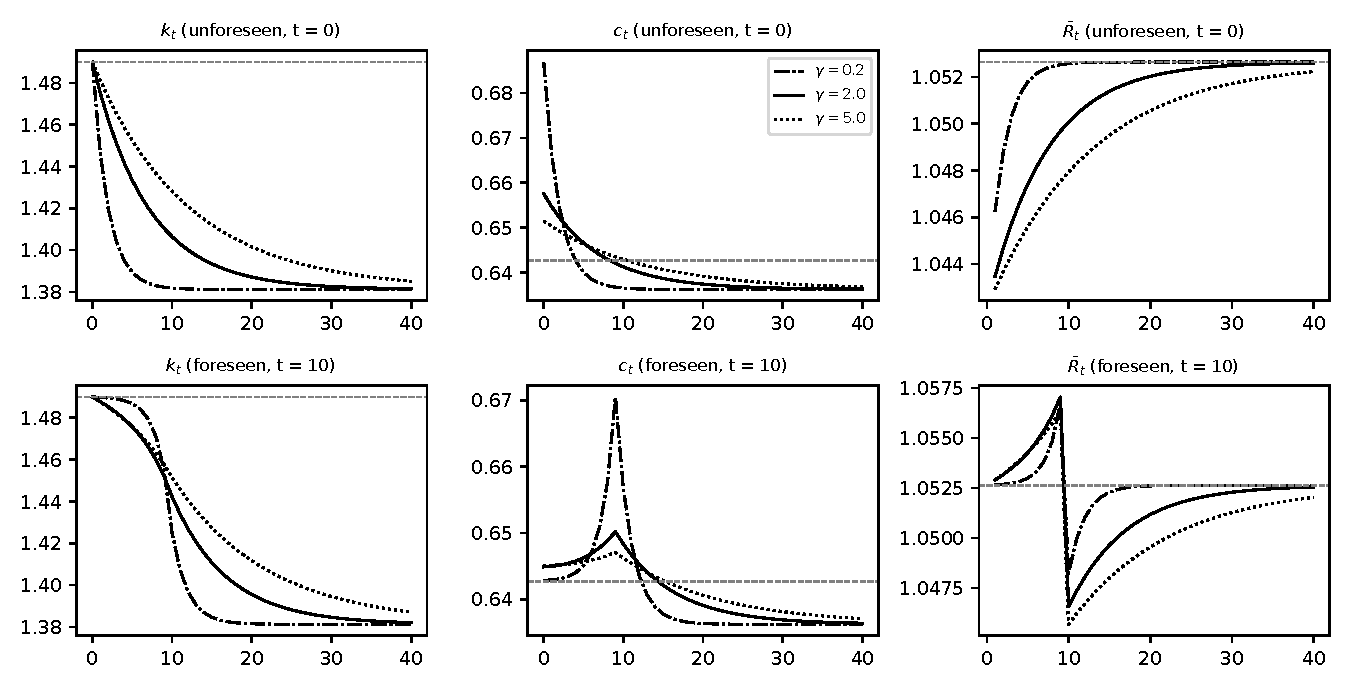
\includegraphics[width=.95\textwidth]{fig/ls11_07_tau_k.pdf}
\captionof{figure}{Exercise 11.7: $\tau_k=.2$ unforeseen at $t=0$ (top) and foreseen for $t=10$ (bottom);
$\gamma=.2$ (dash-dot), 2 (solid), 5 (dotted).}
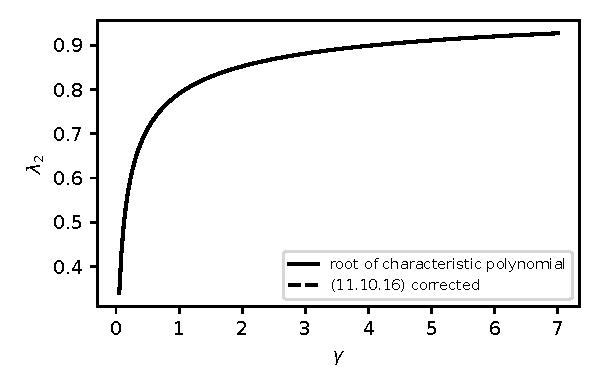
\includegraphics[width=.5\textwidth]{fig/ls11_07_lambda2.pdf}
\captionof{figure}{Exercise 11.7(c): $\lambda_2(\gamma)$, root of the characteristic polynomial vs corrected (11.10.16).}
\end{center}
\end{tcolorbox}

%------- 11.8 -------
\begin{tcolorbox}[evenbox,title={Exercise 11.8 \quad Trade and growth, version II}]
\begin{longquestion}
p.~460. \textbf{Part I.} Consider the problem of the planner in a small economy. When the economy is \underline{closed
to trade}, the planner chooses $\{c_t,k_{t+1}\}_{t=0}^\infty$ to maximize $\sum_{t=0}^\infty\beta^tu(c_t)$, $0<\beta<1$,
$\beta=\frac1{1+\rho}$, $\rho>0$ subject to
\[
c_t+k_t+1=f(k_t)+(1-\delta)k_t,\ \delta\in(0,1)
\]
where

Let $\bar k$ be the steady state value of $k_t$ under the optimal plan.

\textbf{a.} Find a formula for $\bar k$.

\textbf{b.} Assume that $k_0>\bar k$. Describe time paths for $\{c_t,k_{t+1}\}_{t=0}^\infty$ and
$\bar R_{t+1}=(1-\delta)+f'(k_{t+1})$.

\textbf{c.} What is the steady state value of $\bar R_{t+1}$?

\textbf{d.} Is $\bar R_{t+1}$ less or greater than its steady state value when $k_{t+1}>\bar k$?

\textbf{Part II.} \textbf{e.} Now assume that the economy is open to international trade in capital and financial assets.
Assume that there is a fixed world gross rate of return $R=\beta^{-1}$ at which the planner can borrow or
\underline{lend}. In particular, the planner is free to use the following plan. The planner can sell all of its capital
$\bar k_0$ and simply consume the interest payments. Let $\bar k_0$ be the level of initial capital ($\bar k_0>\bar k$)
just before the country opens up to trade just before time 0. Let $\bar k_0$ be the initial capital per capita
$\bar k_0>\bar k$ studied in parts \textbf{a-d}. At time $t=-1$, after $\bar k_0$ was set, trade opens up. At time
$t=-1$, the planner \underline{sells} $\bar k_0$ in exchange for IOU's or bonds from the rest of the world in the amount
$A_{-1}=\bar k_0$.

The bonds $A_{-1}$ are one-period in duration and bear the constant world gross interest rate $R=\beta^{-1}$. After the
sale of $\bar k_0=A_{-1}$, the planner has \underline{zero} capital and so shuts down the technology. Instead, the planner
uses the asset market to smooth consumption. The planner chooses $\{A_{t+1},c_t\}$ to maximize
$\sum_{t=0}^\infty\beta^tu(c_t)$, $0<\beta<1$, $\beta=\frac1{1+\rho}$, $\rho>0$ subject to $c_t+\beta A_{t+1}=A_t$,
$A_0=\bar k_0$. Please find the optimal path for consumption $\{c_t\}$.

\textbf{f.} Compare the path of $(c_t,k_{t+1},\bar R_t)$ that you computed in parts \textbf{a-d} with ``no trade'' with
the part \textbf{e} path ``with trade'' in which the government ``shuts down the home technology'' and lives entirely
from the returns on foreign assets. Can you say which path the representative consumer will prefer?

\textbf{g.} Now return to the economy in part \textbf{e} with $\bar k_0>\bar k$ from part \textbf{d}. Assume that the
planner is free to borrow or lend capital at the fixed gross interest of $\beta^{-1}=1+\rho$, as before. But now assume
the planner chooses the \underline{optimal} amount of $\bar k_0$ to sell off and so does not necessarily sell off the
entire $\bar k_0$ and possibly continues to operate the technology.

\quad\textbf{i)} Find the solution of the planning problem.

\quad\textbf{ii)} Explain why it is optimal not to shut down the technology. \textbf{Hint}: Starting from having shut
the technology down, think of putting a small amount $\epsilon$ of capital into the technology---this earns
$z\epsilon^\alpha$ and costs $\rho\epsilon$ in terms of foregone interest. Because $0<\alpha<1$, $\rho\epsilon<z\epsilon^\alpha$
for small $\epsilon$. Thus, the technology is \underline{very productive} for small $\epsilon$, so it is efficient to use
it.
\end{longquestion}

\textbf{Solution:} \emph{Misprints/omissions.} The constraint ``$c_t+k_t+1$'' should read $c_t+k_{t+1}$. The sentence
``where'' is left unfinished; we use the $u$ and $f$ of exercise 11.6 ($u=c^{1-\gamma}/(1-\gamma)$, $f=zk^\alpha$).

\textbf{(a)} As in 11.6: $\kb=(\alpha z/(\rho+\delta))^{1/(1-\alpha)}$.

\textbf{(b)} Mirror image of 11.6(b): with $k_0>\kb$, $k_t$ falls monotonically to $\kb$. Along the path
$f'(k_{t+1})<\rho+\delta$, so $\Rb_{t+1}<1+\rho$ and $c_{t+1}/c_t=(\beta\Rb_{t+1})^{1/\gamma}<1$: consumption falls
monotonically to $\cb$. $\Rb_{t+1}$ rises monotonically to $1+\rho$.

\textbf{(c)} $1+\rho$. \textbf{(d)} Less, since $f'$ is decreasing.

\textbf{(e)} Lagrangian $\sum_t\beta^t\{u(c_t)+\nu_t[A_t-c_t-\beta A_{t+1}]\}$. FOCs: $u'(c_t)=\nu_t$;
$A_{t+1}$: $-\beta^{t+1}\nu_t+\beta^{t+1}\nu_{t+1}=0$. So $u'(c_t)=u'(c_{t+1})$: consumption is constant. Iterate the
constraint: $A_0=\sum_{t=0}^{T}\beta^tc_t+\beta^{T+1}A_{T+1}$; with no Ponzi scheme, $\beta^TA_T\to0$ and
\[
\sum_t\beta^tc_t=A_0=\kb_0\ \Rightarrow\ \boxed{c_t=(1-\beta)\kb_0=\tfrac{\rho}{1+\rho}\kb_0,\quad A_t=\kb_0 .}
\]
\emph{Timing.} The constraint as printed sets $A_0=\kb_0$, so the bonds bought at $t=-1$ earn no interest between $-1$ and
0. With the timing of 11.6 (bonds bought at $t=-1$ pay $R$ at $t=0$), $A_0=R\kb_0$ and $c=\rho\kb_0$.

\textbf{(f)} The closed path starts high ($c_0$ above $\cb$, since the excess capital is eaten) and declines to
$\cb=f(\kb)-\delta\kb$, with $\Rb<1+\rho$ rising. The sell-all path gives a flat $c=(1-\beta)\kb_0$, with $k=0$. The ranking
depends on $\kb_0$. Selling everything gives up production, and in particular all labour income $w=f(k)-kf'(k)$, in
exchange for interest on $\kb_0$. A sufficient condition for the closed economy to be better: it can keep $k_t=\kb_0$ and
consume $f(\kb_0)-\delta\kb_0$ forever, which beats $(1-\beta)\kb_0$ when $f(\kb_0)/\kb_0\ge\delta+1-\beta$, i.e.\
$\kb_0\le(z/(\delta+1-\beta))^{1/(1-\alpha)}$. For very large $\kb_0$ the net return $f'(k)-\delta$ is negative, and
selling out can win.

\textbf{(g)} (i) With 11.6's timing: sell $\kb_0-k_0$ at $t=-1$, so $B_{-1}=k_0-\kb_0$ (negative: the country lends). The
FOCs of 11.6 Part II apply unchanged: $k_t=\kb$ for all $t\ge0$, $B_t=B_{-1}=\kb-\kb_0<0$ (constant foreign assets), and
\[
c=f(\kb)-\delta\kb+\rho(\kb_0-\kb)\quad\text{for all }t .
\]
(ii) With capital $k$ kept constant and $\kb_0-k$ lent abroad, consumption is
$c(k)=f(k)-(\rho+\delta)k+\rho\kb_0$. Shutting down is $k=0$, $c(0)=\rho\kb_0$. But $c'(k)=f'(k)-(\rho+\delta)\to+\infty$
as $k\to0$: a small $\epsilon$ of capital yields $z\epsilon^\alpha$ and costs $(\rho+\delta)\epsilon$ (foregone interest
\emph{plus depreciation}; the hint's $\rho\epsilon$ omits $\delta\epsilon$, which does not change the argument), and
$z\epsilon^\alpha>(\rho+\delta)\epsilon$ for small $\epsilon$ because $\alpha<1$. $c(k)$ is maximised at $f'(k)=\rho+\delta$,
i.e.\ $k=\kb$, and $c(\kb)-c(0)=f(\kb)-(\rho+\delta)\kb=(1-\alpha)f(\kb)>0$ because $(\rho+\delta)\kb=f'(\kb)\kb=\alpha f(\kb)$.

\begin{tcolorbox}[databox]
$z=1$, $\kb_0=2\kb=2.979913$. Closed: $c_0=1.116898$, $\Rb_1=.969594$ (monotone paths checked). Sell-all:
$c=(1-\beta)\kb_0=.148996$ (or $\rho\kb_0=.156838$ with 11.6's timing). Optimal open: $c=.921064$. Welfare:
sell-all $-134.23<$ closed $-22.175<$ optimal open $-21.714$. Selling everything beats autarky only if
$\kb_0>15.505\kb=23.10$ (\texttt{brentq} on the welfare difference). The sufficient condition above gives
$\kb_0\le(1/.25)^{1/.67}=7.93$. $\arg\max_k[f(k)-(\rho+\delta)k]=\kb$ checked on a grid.
\end{tcolorbox}
\end{tcolorbox}

%------- 11.9 -------
\begin{tcolorbox}[oddbox,title={Exercise 11.9 \quad Linear utility, finite horizon}]
\begin{tcolorbox}[questionbox]
p.~461. Consider a consumer who wants to choose $\{c_t\}_{t=0}^T$ to maximize $\sum_{t=0}^T\beta^tc_t$, $0<\beta<1$ subject
to the intertemporal budget constraint
\[
\sum_{t=0}^TR^{-t}[c_t-y_t]=0,\quad R>1
\]
where $c_t\ge0$ and $y_t>0$ for $t=0,\dots,T$. Here $R>1$ is the gross interest rate $(1+r)$, $r>0$. Assume $R$ is
constant. Here $\{y_t\}_{t=0}^T$ is an exogenous sequence of ``labor income''.

\textbf{a.} Assume that $\beta R<1$. Find the optimal path $\{c_t\}_{t=0}^T$.

\textbf{b.} Assume that $\beta R>1$. Find the optimal path $\{c_t\}_{t=0}^T$.

\textbf{c.} Assume that $\beta R=1$. Find the optimal path $\{c_t\}_{t=0}^T$.
\end{tcolorbox}

\textbf{Solution:} Let $W=\sum_{t=0}^TR^{-t}y_t>0$ and change variables to $d_t=R^{-t}c_t\ge0$. The problem is
\[
\max\sum_{t=0}^T(\beta R)^td_t\quad\text{s.t.}\quad\sum_{t=0}^Td_t=W,\ d_t\ge0,
\]
a linear program over a simplex: put all of $W$ on the date with the largest weight $(\beta R)^t$. KKT: with multiplier
$\lambda$ on the budget and $\nu_t\ge0$ on $c_t\ge0$, $\beta^t-\lambda R^{-t}+\nu_t=0$, $\nu_tc_t=0$. So
$\lambda\ge(\beta R)^t$ for all $t$, with equality where $c_t>0$: $\lambda=\max_t(\beta R)^t$.

\textbf{(a)} $\beta R<1$: $(\beta R)^t$ is largest at $t=0$:
$\boxed{c_0=\sum_{t=0}^TR^{-t}y_t,\ c_t=0\ (t\ge1)}$. The consumer borrows against all future income and consumes at once.

\textbf{(b)} $\beta R>1$: largest at $t=T$: $\boxed{c_T=R^TW=\sum_{t=0}^TR^{T-t}y_t,\ c_t=0\ (t<T)}$. The consumer saves
everything and consumes at the end.

\textbf{(c)} $\beta R=1$: the objective equals $\sum_tR^{-t}c_t=W$ for \emph{every} feasible path. Any $c\ge0$ that
satisfies the budget is optimal, e.g.\ $c_t=y_t$, or the flat path $c_t=W(1-R^{-1})/(1-R^{-(T+1)})$. With linear utility
there is no motive to smooth; a strictly concave $u$ would select the flat path through $u'(c_t)=\beta Ru'(c_{t+1})$.

\begin{tcolorbox}[databox]
$T=5$, $R=1.05$, $y_t$ drawn once from $U(.5,1.5)$ (seed 0), $W=4.994328$. \texttt{linprog}: $\beta=.9$: $c_0=4.9943$;
$\beta=1/R+.02$: $c_5=6.3742=R^5W$; $\beta=1/R$: optimal value $4.994328=W$, also attained by $c=y$ and by a perturbed
feasible path.
\end{tcolorbox}
\end{tcolorbox}

%----------------------------------------------------------------------
\subsection{Reading Paths and Yield Curves (11.10--11.12)}
%----------------------------------------------------------------------

%------- 11.10 -------
\begin{tcolorbox}[evenbox,title={Exercise 11.10 \quad Term structure of interest rates}]
\begin{tcolorbox}[questionbox]
p.~462. This problem assumes the following environment. A representative consumer has preferences ordered by
$\sum_{t=0}^\infty\beta^tu(c_t)$, $0<\beta<1$, $\beta=\frac1{1+\rho}$, $\rho>0$, where $c_t$ is the consumption per worker
and where $u(c)=\frac{c^{1-\gamma}}{1-\gamma}$ if $\gamma>0$ and $\gamma\ne1$, $\log(c)$ if $\gamma=1$. The technology is
$y_t=f(k_t)=zk_t^\alpha$, $0<\alpha<1$, $z>0$, where $y_t$ is the output per unit labor and $k_t$ is capital per unit labor,
$y_t=c_t+x_t+g_t$, $k_{t+1}=(1-\delta)k_t+x_t$, $0<\delta<1$, where $x_t$ is gross investment per unit of labor and $g_t$
is government expenditures per unit of labor. The government finances its expenditures by levying some combination of a
flat rate tax $\tau_{ct}$ on the value of consumption goods purchased at $t$, a flat rate tax $\tau_{nt}$ on the value of
labor earnings at $t$, a flat rate tax $\tau_{kt}$ on earnings from capital at $t$ and a lump sum tax of $\tau_{ht}$ in time
$t$ consumption goods per worker at time $t$. Define
$\bar R_{t+1}=\frac{(1+\tau_{ct})}{(1+\tau_{ct+1})}\left[1+(1-\tau_{kt+1})(f'(k_{t+1}-\delta)\right]$.

\textbf{a.} Recall that we can represent $q^0_t=q^0_0m_{0,1}m_{1,2}\cdots m_{t-1,t}$ where
$m_{t-1,t}=\frac{q^0_t}{q^0_{t-1}}$ and $m_{t-1,t}\equiv\exp(-r_{t-1,t})\approx\frac1{1+r_{t-1,t}}$. Further, recall that
the $t$ period long yield satisfies $q^0_t=\exp(-tr_{0,t})$ and $r_{0,t}=\frac1t[r_{0,1}+r_{1,2}+\dots+r_{t-1,t}]$. Now
suppose that at $t=0$, $k_0=\bar k$, where $\bar k$ is the steady state appropriate for an economy with constant
$g_t=\bar g>0$ and all expenditures are financed by lump sum taxes. Find $q^0_t$ for this economy.

\textbf{b.} Plot $r_{t-1,t}$ for this economy for $t=1,2,\dots,10$.

\textbf{c.} Plot $r_{0,t}$ for this economy for $t=1,2,\dots,10$ (this is what Bloomberg plots).

\textbf{d.} Now assume that at time 0, starting from $k_0=\bar k$ for the steady state you computed in part a, the
government unexpectedly and permanently raises the tax rate on income from capital $\tau_{kt}=\tau_k>0$ to a positive
rate.

\quad\textbf{i)} Plot $r_{t-1t}$ for this economy for $t=1,2,\dots,10$. Explain how you got this outcome.

\quad\textbf{ii)} Plot $r_{0,t}$ for this economy for $t=1,2,\dots,10$. Explain how you got this outcome.
\end{tcolorbox}

\textbf{Solution:} \emph{Misprint.} In the definition of $\Rb_{t+1}$, ``$f'(k_{t+1}-\delta)$'' should be
$f'(k_{t+1})-\delta$, as in (11.6.8e). We use $r_{t-1,t}\equiv-\log m_{t-1,t}$ exactly.

\textbf{(a)} With lump-sum finance and $k_0=\kb$, the equilibrium is stationary (as in 11.5(c)): $c_t=\cb$, $k_t=\kb$. By
(11.6.8b), $q^0_t=\beta^tu'(\cb)/(1+\tau_c)$; normalising $q^0_0=1$,
\[
q^0_t=\beta^t,\qquad m_{t-1,t}=\beta .
\]

\textbf{(b)} $r_{t-1,t}=-\log\beta=\log(1+\rho)\approx\rho$ for every $t$: a flat line.

\textbf{(c)} $r_{0,t}=t^{-1}\sum_{s=1}^tr_{s-1,s}=-\log\beta$: the yield curve is flat.

\textbf{(d)} After the surprise, the economy follows the path of 11.7(b): $k$ declines from $\kb$ to $\hat k$, $c$ jumps up
and declines, and $\Rb_{t+1}<1+\rho$ rises back to $1+\rho$.

(i) By (11.6.8f) with $\tau_c$ constant,
$m_{t,t+1}=\beta u'(c_{t+1})/u'(c_t)=1/\Rb_{t+1}$, so
\[
r_{t,t+1}=\log\Rb_{t+1}=\log\big[1+(1-\tau_k)(f'(k_{t+1})-\delta)\big]=-\log\beta+\gamma\log\frac{c_{t+1}}{c_t}.
\]
Since $c$ falls along the transition, short rates are below $-\log\beta$. Since the fall slows down as $k\to\hat k$, they rise
monotonically toward $-\log\beta$. Equivalently: $k_{t+1}$ falls toward $\hat k$, so $f'(k_{t+1})$ rises toward
$\delta+\rho/(1-\tau_k)$.

(ii) $r_{0,t}$ is the running average of the short rates. The short rates increase, so the yield curve slopes upward, lies
below the short-rate curve for $t\ge2$, and converges to $-\log\beta$ at long maturities.

\begin{tcolorbox}[databox]
Benchmark, $\gb=.2$, $\tau_k=.2$. (a)--(c) $q_t=\beta^t$, $r=-\log\beta=.051293$ (checked on the Newton path).
(d) Check: $\log(q_t/q_{t+1})=\log\Rb_{t+1}$ on the Newton path.

\smallskip
\resizebox{\linewidth}{!}{%
\begin{tabular}{@{}lcccccccccc@{}}
\toprule
$t$ & 1 & 2 & 3 & 4 & 5 & 6 & 7 & 8 & 9 & 10\\
\midrule
$r_{t-1,t}$ & .04255 & .04370 & .04469 & .04556 & .04632 & .04698 & .04755 & .04805 & .04848 & .04886\\
$r_{0,t}$ & .04255 & .04312 & .04365 & .04413 & .04457 & .04497 & .04534 & .04568 & .04599 & .04627\\
\bottomrule
\end{tabular}}
\end{tcolorbox}

\begin{center}
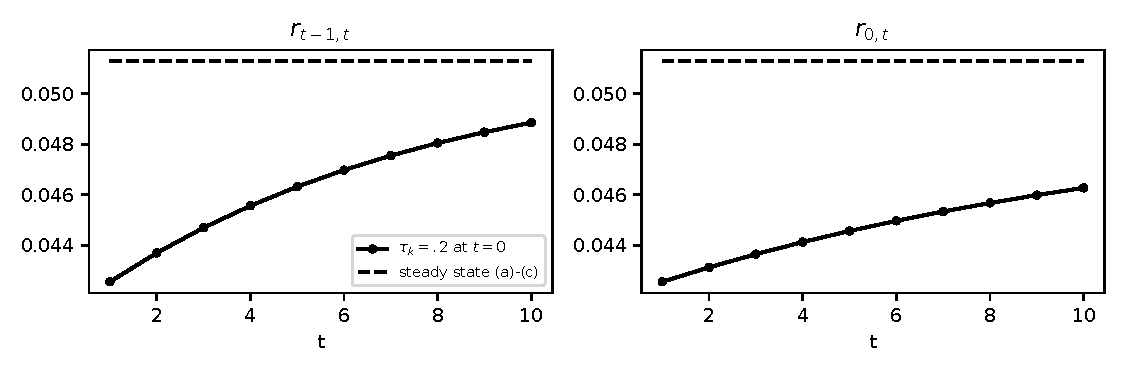
\includegraphics[width=.8\textwidth]{fig/ls11_10_yields.pdf}
\captionof{figure}{Exercise 11.10: short rates and yields; flat at $-\log\beta$ in (a)--(c), rising after the capital tax in (d).}
\end{center}
\end{tcolorbox}

%------- 11.11 -------
\begin{tcolorbox}[oddbox,title={Exercise 11.11 \quad A rising consumption path}]
\begin{tcolorbox}[questionbox]
p.~463. This problem assumes the same economic environment as the previous exercise i.e, the ``growth model'' with fiscal
policy. Suppose that you observe the path for consumption per capita in figure 11.1. Say what you can about the likely
behavior over time of $k_t$, $\bar R_t=[1+(1-\tau_{kt})(f'(k_t)-\delta)]$, $g_t$ and $\tau_{kt}$. (You are free to make up
any story that is consistent with the model.)

\smallskip
\emph{[Figure 11.1: consumption per capita $c_t$ starts at a positive level at $t=0$ and rises at a decreasing rate.]}
\end{tcolorbox}

\textbf{Solution:} Keep $\tau_c$ constant. Then (11.6.9) gives
\[
\log\frac{c_{t+1}}{c_t}=\frac1\gamma\big[\log\beta+\log\Rb_{t+1}\big].
\]
In figure 11.1 consumption growth is positive and declining, so $\Rb_{t+1}>1+\rho$ and $\Rb_{t+1}$ falls toward $1+\rho$.
With $\Rb_t=1+(1-\tau_{kt})(f'(k_t)-\delta)$ and a constant $\tau_k$, a falling $\Rb$ means a falling $f'(k_t)$, i.e.\
\emph{rising capital}, converging to its steady state. Two consistent stories:
\begin{enumerate}[label=(\roman*)]
\item \emph{No policy change}: constant $g_t$ and $\tau_{kt}$, and the economy starts with $k_0$ below its steady state
(the standard transition of 11.6(b) and 11.14(c)).
\item \emph{A surprise capital-tax cut}: the economy was in the steady state with $\tau_k>0$. At $t=0$ the government
unexpectedly and permanently sets $\tau_{kt}=0$ (constant $g_t$, lump-sum taxes absorb the revenue loss). The after-tax
return at the old capital stock jumps above $1+\rho$; the household invests; $k$ rises to the higher steady state
$f'(k)=\rho+\delta$; $\Rb$ falls back to $1+\rho$.
\end{enumerate}
In both, $g_t$ is constant; $\tau_{kt}$ is constant from $t=0$ on (in (ii), at a lower level than before $t=0$). What is
\emph{not} consistent: a surprise permanent change in $g$ alone (consumption shifts once and stays flat, 11.5(c)); an
anticipated future rise in $g$ (consumption falls, 11.17).

\begin{tcolorbox}[databox]
Checked on the Newton paths (first 40 periods): $\Delta c_t>0$ and decreasing; $\Rb_t>1+\rho$ and decreasing.
(i) $k_0=.5\kb$: $c_0=.4665\to.6426$, $k_0=.7450\to1.4900$, $\Rb_1=1.1718$. (ii) $\tau_k=.2\to0$ at $t=0$:
$c_0=.6204\to.6426$, $k_0=1.3812\to1.4900$, $\Rb_1=1.0638$.
\end{tcolorbox}

\begin{center}
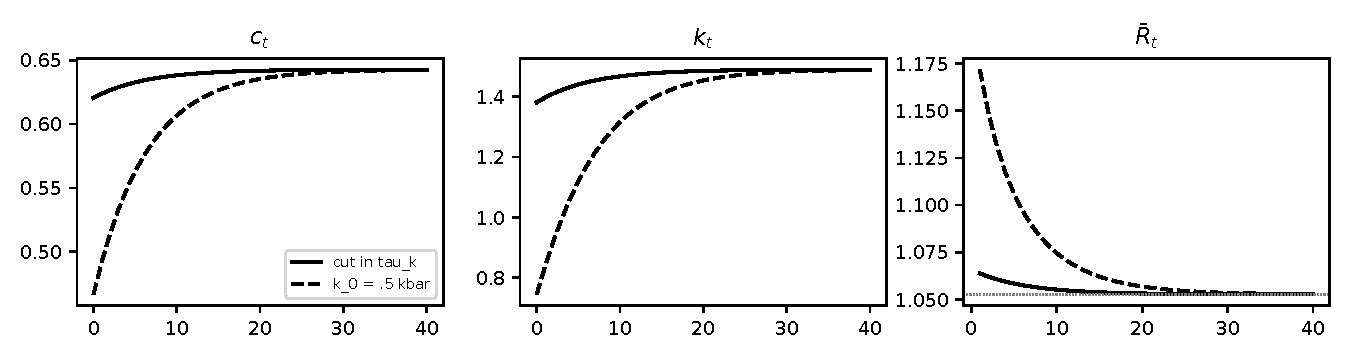
\includegraphics[width=.9\textwidth]{fig/ls11_11_rising_c.pdf}
\captionof{figure}{Exercise 11.11: surprise cut in $\tau_k$ (solid) and $k_0=.5\kb$ (dashed).}
\end{center}
\end{tcolorbox}

%------- 11.12 -------
\begin{tcolorbox}[evenbox,title={Exercise 11.12 \quad Flat, then a drop, then a decline}]
\begin{tcolorbox}[questionbox]
p.~463. Assume the same economic environment as in the previous two problems. Assume that someone has observed the time
path for $c_t$ in figure 11.2:

\smallskip
\emph{[Figure 11.2: $c_t$ is constant from $t=0$ until $t=12$, drops discretely at $t=12$, and then declines at a
decreasing rate toward a lower level.]}

\textbf{a.} Describe a consistent set of assumptions about the fiscal policy that explains this time path for $c_t$. In
doing so, please distinguish carefully between changes in taxes and expenditures that are \underline{foreseen} versus
\underline{unforeseen}.

\textbf{b.} Describe what is happening to $k_t$, $\bar R_t$ and $g_t$ over time. Make whatever assumptions you must to get
a complete but consistent story - here ``consistent'' means ``consistent with the economic environment we have
assumed''.
\end{tcolorbox}

\textbf{Solution:}

\textbf{(a)} \emph{Before $t=12$.} Constant consumption means $\Rb_{t+1}=1+\rho$ by (11.6.9): the economy sits in a
steady state. Nothing that happens at or after $t=12$ was known before $t=12$: a foreseen change would move consumption
before it occurs (section 11.9). So the news arrives at $t=12$ and is \emph{unforeseen}.

\emph{At $t=12$.} A discrete drop is a negative wealth effect: the present value of taxes jumps (higher government
spending). \emph{After $t=12$.} Gradual decline means $\Rb_{t+1}<1+\rho$ for a while, rising back to $1+\rho$.
Two consistent stories:
\begin{itemize}[itemsep=2pt]
\item \textbf{A (unforeseen news of a foreseen change).} At $t=12$ the government announces, unexpectedly, a permanent rise
in $g$ from $t=22$ on, financed by lump-sum taxes. From $t=12$ on the rise is foreseen. Consumption drops at 12 (wealth
effect) and then declines smoothly to $\cb-\Delta g$. This is figure 11.9.1 shifted to start at $t=12$.
\item \textbf{B (unforeseen immediate change with a distorting tax).} At $t=12$, $g$ rises permanently and at once and the
government raises $\tau_k$ permanently (lump sums cover the rest). Consumption drops at 12, by a little less than
$\Delta g$ because the tax increase also makes the household run down capital. It then declines as $k$ falls toward the
lower steady state of the higher $\tau_k$.
\end{itemize}

\textbf{(b)} Story A: $g=.2$ until $t=21$, $.4$ from $t=22$; $\tau_k=0$. After 12, capital is \emph{built up} until
$t=22$ and then run down back to $\kb$ (the steady state does not depend on $g$). $\Rb$ falls below $1+\rho$ after 12, is
lowest at $t=22$ when $k$ peaks, and then rises back to $1+\rho$.
Story B: $g$ jumps at 12; $k$ declines monotonically from $\kb$ to $\hat k$; $\Rb$ drops below $1+\rho$ at 13 and rises
back. The two stories differ in the path of $k$ (up then down in A; down in B), which data on investment could separate.

\begin{tcolorbox}[databox]
Benchmark; A: $g=.2\to.4$ at $t=22$, announced at 12; B: $g=.2\to.4$ and $\tau_k=0\to.2$ at 12. Both reproduce the shape
(checked: $c_{12}<c_{11}$ and $c$ strictly decreasing from 12 to 51).
A: $c_{11}=.6426$, $c_{12}=.6092$, $c_{40}=.4518$; $\max_tk_t=2.0985$ (at $t=22$); $\Rb_{13}=1.0489$.
B: $c_{12}=.4548$, $c_{40}=.4370$; $k_{40}=1.3854$; $\Rb_{13}=1.0432$.
\end{tcolorbox}

\begin{center}
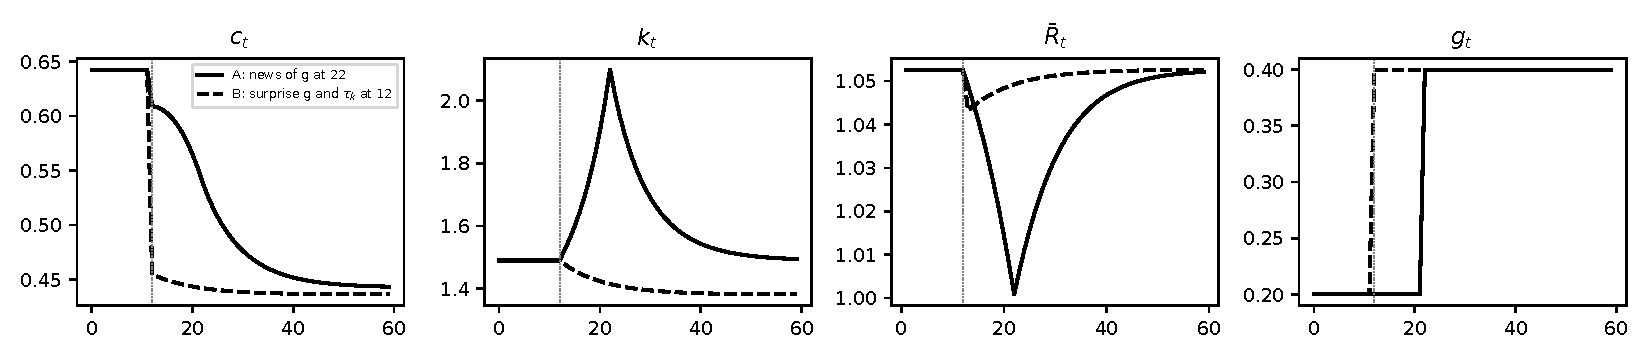
\includegraphics[width=\textwidth]{fig/ls11_12_stories.pdf}
\captionof{figure}{Exercise 11.12: story A (solid) and story B (dashed); vertical line at $t=12$.}
\end{center}
\end{tcolorbox}

%----------------------------------------------------------------------
\subsection{Linear Utility, a Transition with $g$, Yield Curves and News (11.13--11.17)}
%----------------------------------------------------------------------

%------- 11.13 -------
\begin{tcolorbox}[oddbox,title={Exercise 11.13 \quad Optimal growth with linear utility}]
\begin{tcolorbox}[questionbox]
p.~464. Consider the optimal growth model with a representative consumer with preferences $\sum_{t=0}^\infty\beta^tc_t$,
$0<\beta<1$, with technology
\[
c_t+k_{t+1}=f(k_t)+(1-\delta)k_t,\quad\delta\in(0,1),\qquad c_t\ge0,\quad k_0>0\text{ given}
\]
\[
f'>0,\quad f''<0,\quad\lim_{k\to0}f'(k)=+\infty,\quad\lim_{k\to+\infty}f'(k)=0 .
\]
Let $\bar k$ be the steady state capital stock for the optimal planning problem.

\textbf{a.} For $k_0$ given, formulate and solve the optimal planning problem.

\textbf{b.} For $k_0>\bar k$, describe the optimal time path of $\{c_t,k_{t+1}\}_{t=0}^\infty$.

\textbf{c.} For $k_0<\bar k$, describe the optimal path of $\{c_t,k_{t+1}\}_{t=0}^\infty$.

\textbf{d.} Let the \underline{saving rate} $s_t$ be defined as the $s_t$ that satisfies
$k_{t+1}=s_tf(k_t)+(1-\delta)k_t$. Here $s_t$ in general varies along a $\{c_t,k_{t+1}\}$ sequence. Say what you can
about how $s_t$ varies as a function of $k_t$.
\end{tcolorbox}

\textbf{Solution:} Let $Y(k)=f(k)+(1-\delta)k$ (increasing). Define $\kb$ by $f'(\kb)=\rho+\delta$.

\textbf{(a)} $\max\sum_t\beta^t[Y(k_t)-k_{t+1}]$ subject to $0\le k_{t+1}\le Y(k_t)$ (the upper bound is $c_t\ge0$).
Regroup the terms by $k_t$:
\[
\sum_{t\ge0}\beta^t[Y(k_t)-k_{t+1}]=Y(k_0)+\sum_{t\ge1}\beta^t\varphi(k_t),\qquad\varphi(k)\equiv Y(k)-\frac k\beta .
\]
$\varphi'(k)=f'(k)+1-\delta-1/\beta=f'(k)-(\rho+\delta)$, so $\varphi$ is strictly concave, increasing on $(0,\kb)$ and
maximised at $\kb$. The objective is separable in the $k_t$; only the constraints $k_{t+1}\le Y(k_t)$ link dates. Claim:
\[
\boxed{k_{t+1}=\min\{Y(k_t),\kb\},\qquad c_t=\max\{0,\,Y(k_t)-\kb\}.}
\]
Proof. Let $\{k^\ast_t\}$ be this path and $\{k_t\}$ any feasible path, both from $k_0$. (1) If $k^\ast_t<\kb$ then
$k_t\le k^\ast_t$. By induction: if $k^\ast_t<\kb$, then $k^\ast_t=Y(k^\ast_{t-1})$ with $k^\ast_{t-1}<\kb$, and
$k_t\le Y(k_{t-1})\le Y(k^\ast_{t-1})=k^\ast_t$ since $k_{t-1}\le k^\ast_{t-1}$ and $Y$ is increasing. (2) Hence at dates
with $k^\ast_t<\kb$, $\varphi(k_t)\le\varphi(k^\ast_t)$ because $\varphi$ is increasing below $\kb$. At dates with
$k^\ast_t=\kb$, $\varphi(k^\ast_t)=\max\varphi\ge\varphi(k_t)$. Summing, $\{k^\ast_t\}$ is optimal (uniquely, by strict
concavity of $\varphi$ on the dates where it binds). Value for $Y(k)\ge\kb$:
$V(k)=Y(k)-\kb+\beta\cb/(1-\beta)$ with $\cb=f(\kb)-\delta\kb$.

The Euler equation explains the solution: with linear utility, $c_t>0$ requires $\beta[f'(k_{t+1})+1-\delta]=1$, i.e.\
$k_{t+1}=\kb$. If the return exceeds $1/\beta$ ($k_{t+1}<\kb$) the planner saves everything; if it falls short, it
consumes the excess.

\textbf{(b)} $k_0>\kb$: $Y(k_0)>\kb$, so $c_0=Y(k_0)-\kb$ (the excess capital is eaten at once); then $k_t=\kb$ and
$c_t=\cb$ for $t\ge1$.

\textbf{(c)} $k_0<\kb$: while $Y(k_t)<\kb$, $c_t=0$ and $k_{t+1}=Y(k_t)$ (grow as fast as possible). At the first date
$\tau$ with $Y(k_\tau)\ge\kb$: $c_\tau=Y(k_\tau)-\kb\ge0$ and $k_{\tau+1}=\kb$; then $\cb$ forever. This is a ``most rapid
approach'' path: with linear utility the elasticity of intertemporal substitution is infinite ($\gamma=0$, so $\lambda_2=0$
in (11.10.16)).

\textbf{(d)} $s_t=[k_{t+1}-(1-\delta)k_t]/f(k_t)$. With the policy of (a), let $\underline k$ solve $Y(\underline k)=\kb$.
\[
s(k)=\begin{cases}1, & k\le\underline k,\\[2pt]\dfrac{\kb-(1-\delta)k}{f(k)}, & k\ge\underline k .\end{cases}
\]
$s$ is continuous at $\underline k$ ($s=1$). On $[\underline k,\infty)$,
$s'(k)=\{-(1-\delta)f-[\kb-(1-\delta)k]f'\}/f^2$. Where the numerator of $s$ is positive, both terms are negative. Where it
is negative, $-(1-\delta)f+((1-\delta)k-\kb)f'=-(1-\delta)(f-kf')-\kb f'<0$, since $f-kf'>0$. So $s$ equals 1 for low $k$
and then decreases strictly. At the steady state $s(\kb)=\delta\kb/f(\kb)$ ($=\delta\alpha/(\rho+\delta)$ for
Cobb--Douglas). $s<0$ (dissaving, consuming out of capital) for $k>\kb/(1-\delta)$.

\begin{tcolorbox}[databox]
Benchmark $f=k^{.33}$: $\kb=1.489956$, $\cb=.842645$, $\underline k=.733812$, $s(\kb)=.261250$, $s<0$ for
$k>1.862446$. Grid VFI (1501 points including $\kb$; 534 iterations) confirms: policy $=\kb$ whenever $Y(k)\ge\kb$, $c=0$
(up to grid spacing) otherwise, and $V(k)=Y(k)-\kb+\beta\cb/(1-\beta)$ on the reachable region. From $k_0=.05$:
$k=.05,.4121,1.0760,1.49,\dots$; $c=0,0,.3954,.8426,\dots$
\end{tcolorbox}

\begin{center}
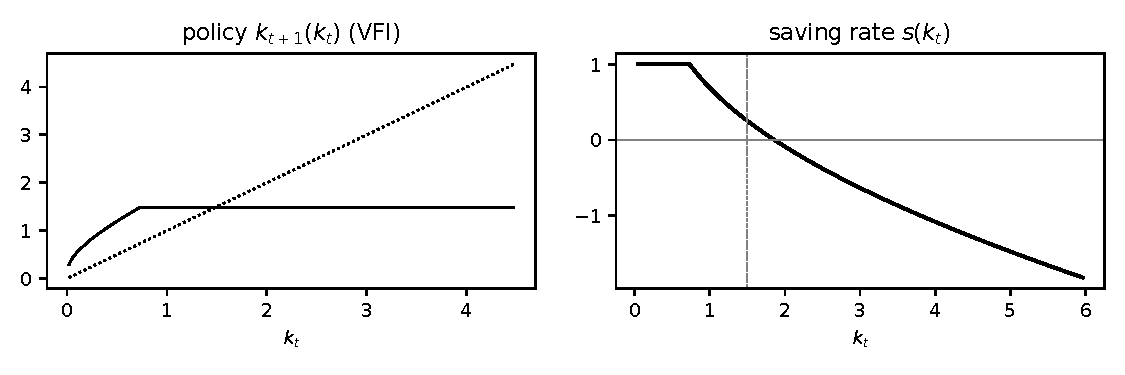
\includegraphics[width=.8\textwidth]{fig/ls11_13_linear.pdf}
\captionof{figure}{Exercise 11.13: VFI policy function and the saving rate $s(k)$ (dashed: $\kb$).}
\end{center}
\end{tcolorbox}

%------- 11.14 -------
\begin{tcolorbox}[evenbox,title={Exercise 11.14 \quad Transitions with and without government purchases}]
\begin{tcolorbox}[questionbox]
p.~465. A representative consumer has preferences over consumption streams ordered by $\sum_{t=0}^\infty\beta^tu(c)$,
$0<\beta<1$, where $\beta\equiv\frac1{1+\rho}$, $c_t$ is consumption per worker, $\gamma>0$, and
$u(c)=\frac{c^{1-\gamma}}{1-\gamma}$ if $\gamma>0$ and $\gamma\ne1$, $\log(c)$ if $\gamma=1$. The consumer supplies one unit
of labor inelastically. The technology is $y_t=f(k_t)=zk_t^\alpha$, $0<\alpha<1$ where $y_t$ is output per worker, $k_t$
is capital per worker, $x_t$ is gross investment per worker, $g_t$ = government expenditures per worker, and
$y_t=c_t+x_t+g_t$, $k_{t+1}=(1-\delta)k_t+x_t$, $0<\delta<1$.

The government finances its expenditure stream $\{g_t\}$ by levying a stream of flat rate taxes $\{\tau_{ct}\}$ on the value
of the consumption good purchased at $t$, a stream of flat rate taxes $\{\tau_{kt}\}$ on earnings from capital at $t$,
and a stream of lump sum taxes $\{\tau_{ht}\}$. Let $\{q_t,q_t\eta_t,q_tw_t\}_{t=0}^\infty$ be a \emph{price system}, where
$q_t$ is the price of time $t$ consumption and investment goods, $q_t\eta_t$ is the price of renting capital at time $t$,
and $q_tw_t$ is the price of renting labor at time $t$. All trades occur at time 0 and all prices are measured in units of
the time 0 consumption good. The initial capital stock $k_0$ is given.

\textbf{a.} Define a competitive equilibrium with taxes and government purchases.

\textbf{b.} Assume that $g_t=0$ for all $t\ge0$ and that all taxes are also zero. Find the value $\bar k$ of the steady
state capital per worker. Find a formula for the saving rate $\frac{x_t}{f(k_t)}$ at the steady state value of the
capital stock.

\textbf{c.} Suppose that the initial capital stock $k_0=.5\bar k$, so that the economy starts below its steady state
level. Describe (i.e., draw graphs showing) the time paths of $\{c_t,k_{t+1},\bar R_{t+1}\}_{t=0}^\infty$ where
$\bar R_{t+1}\equiv[(1-\delta)+f'(k_{t+1})]$.

\textbf{d.} Starting from the same initial $k_0$ as in part \textbf{c}, assume now that $g_t=\bar g=\phi f(k_0)>0$ for
all $t\ge0$ where $\phi\in(0,1-\delta)$. Assume that the government finances its purchases by imposing lump sum taxes.
Describe (i.e., draw graphs) showing the time paths of $\{c_t,k_{t+1},\bar R_{t+1}\}_{t=0}^\infty$ and compare them to the
outcomes that you obtained in part \textbf{c}. What outcomes differ? What outcomes, if any, are identical across the two
economies? Please explain.

\textbf{e.} Starting from the same initial $k_0$ assumed in part \textbf{c}, assume now that $g_t=\bar g=\phi f(k_0)>0$
for all $t\ge0$ where $\phi\in(0,1-\delta)$. Assume that the government must now finance these purchases by imposing a
time-invariant tax rate $\bar\tau_k$ on capital each period. The government \emph{cannot} impose lump sum taxes or any
other kind of taxes to balance its budget. Please describe how to find a competitive equilibrium.
\end{tcolorbox}

\textbf{Solution:}

\textbf{(a)} A competitive equilibrium is a price system $\{q_t,\eta_t,w_t\}$, a policy
$\{g_t,\tau_{ct},\tau_{kt},\tau_{ht}\}$ with
$\sum_tq_tg_t=\sum_tq_t[\tau_{ct}c_t+\tau_{kt}(\eta_t-\delta)k_t+\tau_{ht}]$, and an allocation $\{c_t,x_t,k_{t+1}\}$ such
that: the household maximises $\sum_t\beta^tu(c_t)$ subject to
$\sum_tq_t[(1+\tau_{ct})c_t+x_t]\le\sum_tq_t[\eta_tk_t-\tau_{kt}(\eta_t-\delta)k_t+w_t-\tau_{ht}]$ and
$k_{t+1}=(1-\delta)k_t+x_t$, $k_0$ given; the firm sets $\eta_t=f'(k_t)$, $w_t=f(k_t)-k_tf'(k_t)$; and
$c_t+x_t+g_t=f(k_t)$. The equilibrium conditions are (11.6.3), (11.6.1), $k_0$ and (11.5.3).

\textbf{(b)} $f'(\kb)=\rho+\delta$: $\kb=(\alpha z/(\rho+\delta))^{1/(1-\alpha)}$. At the steady state $x=\delta\kb$ and
$\alpha z\kb^{\alpha-1}=\rho+\delta$ gives $\kb/f(\kb)=\alpha/(\rho+\delta)$, so
\[
\frac{x}{f(\kb)}=\frac{\delta\kb}{f(\kb)}=\frac{\alpha\delta}{\rho+\delta}.
\]

\textbf{(c)} As in 11.6(b): $k_t$ and $c_t$ rise monotonically to $\kb$ and $\cb=f(\kb)-\delta\kb$; $\Rb_{t+1}>1+\rho$ and
falls monotonically to $1+\rho$ (figure).

\textbf{(d)} Lump-sum finance leaves the Euler equation unchanged and shifts feasibility by $\gb$:
$u'(c_t)=\beta u'(c_{t+1})[f'(k_{t+1})+1-\delta]$, $c_t=f(k_t)+(1-\delta)k_t-\gb-k_{t+1}$.
\begin{itemize}[itemsep=2pt]
\item \emph{Identical}: the steady-state capital $\kb$ (the Euler equation does not contain $g$), hence the steady-state
$\Rb=1+\rho$, $\eta=f'(\kb)$, $w$ and saving rate; the mapping (11.6.9) from $\Rb$ to consumption growth; and
the irrelevance of the timing of lump-sum taxes.
\item \emph{Different}: the level of consumption (lower by exactly $\gb$ in the steady state; by less than $\gb$ at first,
because investment also falls), and the transition. With $g>0$ capital accumulates \emph{more slowly} and $\Rb$ stays
higher for longer. Reason: the feedback coefficient depends on $A/\gamma=\beta c|f''|/\gamma$ (see 11.7(c)); lower
consumption means lower $A$ and a $\lambda_2$ closer to 1. Intuitively, $-u''/u'=\gamma/c$: when consumption is low, a
given cut in consumption is a larger proportional cut and more costly in utility, so the household is less willing to
sacrifice consumption to build capital.
\end{itemize}

\textbf{(e)} With no lump-sum taxes, the budget $\sum_tq_t\bar\tau_k(f'(k_t)-\delta)k_t=\sum_tq_t\gb$ must hold at the
equilibrium prices. Algorithm:
\begin{enumerate}[label=\arabic*.]
\item Guess $\bar\tau_k$. Terminal steady state: $f'(\hat k)=\delta+\rho/(1-\bar\tau_k)$.
\item Shoot (or Newton) on (11.6.3) with $\tau_{kt}=\bar\tau_k$, $g_t=\gb$, from $k_0$ to $\hat k$: this gives
$\{c_t,k_{t+1}\}$.
\item Prices $q_t=\beta^tu'(c_t)/(1+\tau_c)$, $\eta_t=f'(k_t)$ (normalise $q_0=1$).
\item Compute the gap $G(\bar\tau_k)=\sum_tq_t\bar\tau_k(f'(k_t)-\delta)k_t-\gb\sum_tq_t$ (the $t=0$ term taxes the given
$k_0$ and does not distort).
\item Update $\bar\tau_k$ by bisection until $G=0$, taking the smallest root (revenue has a Laffer curve); if $\max G<0$, no
equilibrium exists.
\end{enumerate}

\begin{tcolorbox}[databox]
Benchmark with $g=0$ in (c); $\phi=.1$, so $\gb=\phi f(k_0)=.090742$ in (d)--(e). $\phi$ is chosen so that (e) has an
equilibrium: the steady-state capital-tax revenue cannot exceed $.146$ (see 11.2), and the book's range
$\phi\in(0,1-\delta)$ allows values that cannot be financed.
(b) $\kb=1.489956$, $x/f=.261250$. (c) $k_0=.744978$: $c_0=.647540$, $\Rb_1=1.166272$.
(d) $c_0=.565017$, $\Rb_1=1.168648$; $k_{10}=1.342656$ vs $1.360230$ without $g$ ($k_t$ lower and $\Rb_{t+1}$ higher at every
date up to 40, checked); same $\kb$ and limiting $\Rb$.
(e) $\bar\tau_k=.641199$, $\hat k=.929016$, $c_0=.649316$, $k_{10}=.866239$.
\end{tcolorbox}

\begin{center}
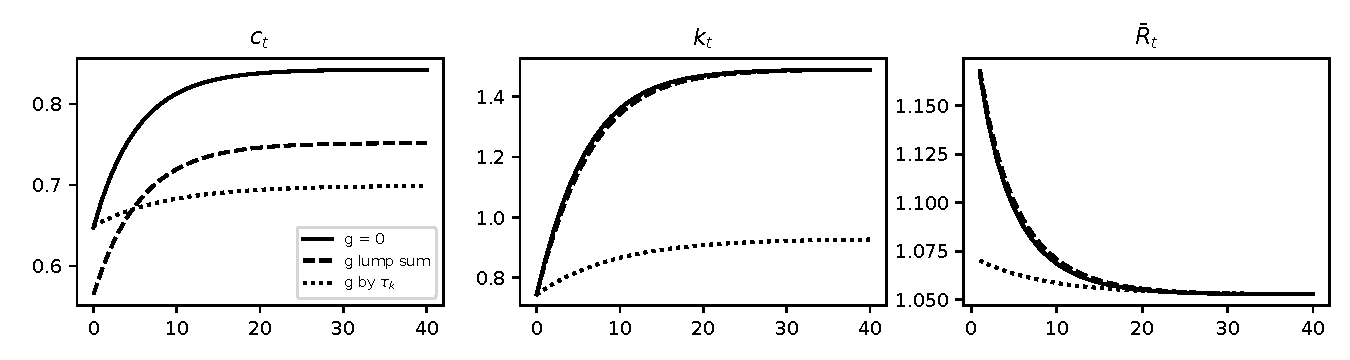
\includegraphics[width=.9\textwidth]{fig/ls11_14_paths.pdf}
\captionof{figure}{Exercise 11.14: $g=0$ (solid), $g$ by lump sums (dashed), $g$ by a constant $\bar\tau_k$ (dotted).}
\end{center}
\end{tcolorbox}

%------- 11.15 -------
\begin{tcolorbox}[oddbox,title={Exercise 11.15 \quad Reading a yield curve}]
\begin{tcolorbox}[questionbox]
p.~466. The structure of the economy is identical to that described in the previous exercise. Let $r_{0,t}$ be the yield
to maturity on a $t$ period bond at time 0, $t=1,2,\dots$. At time 0, Bloomberg reports the term structure of interest
rates in figure 11.3. Please say what you can about the evolution of $\{c_t,k_{t+1}\}$ in this economy. Feel free to make
any assumptions you need about fiscal policy $\{g_t,\tau_{kt},\tau_{ct},\tau_{ht}\}_{t=0}^\infty$ to make your answer
coherent.

\smallskip
\emph{[Figure 11.3: the yield to maturity $r_{0,t}$ as a function of $t=0,\dots,40$ starts low and rises at a decreasing
rate.]}
\end{tcolorbox}

\textbf{Solution:} From (11.6.8f),
\[
r_{t,t+1}=-\log\beta+\gamma\log\frac{c_{t+1}}{c_t}+\log\frac{1+\tau_{c,t+1}}{1+\tau_{ct}},\qquad
r_{0,t}=\frac1t\sum_{s=0}^{t-1}r_{s,s+1}.
\]
A rising, concave yield curve means that short rates rise over time and settle down. Once policy is constant the long rate
must converge to $-\log\beta$, so the short rates are below $-\log\beta$ and rising. With $\tau_c$ constant this means
$c_{t+1}<c_t$: \emph{consumption falls over time at a decreasing rate} and converges. Because
$r_{t,t+1}=\log\Rb_{t+1}=\log[1+(1-\tau_k)(f'(k_{t+1})-\delta)]<\log(1+\rho)$, $f'(k_{t+1})$ is below its steady-state
value: \emph{capital is above its steady state and falling}. Consistent stories:
\begin{enumerate}[label=(\roman*)]
\item a surprise permanent rise in $\tau_k$ at $t=0$, starting from the old steady state (11.10(d)): $c$ jumps up at 0 and
then declines, $k$ declines to the new, lower steady state;
\item constant policy and $k_0$ above its steady state (e.g.\ capital inherited from an earlier regime with higher saving):
$c$ and $k$ decline monotonically.
\end{enumerate}
A path of \emph{rising} consumption taxes would also raise short rates (the last term); we do not need it.

\begin{tcolorbox}[databox]
Checked on the Newton paths: $r_{0,t}$ increasing and concave for $t\le40$, $c$ and $k$ decreasing.
(i) $\tau_k=.2$ at 0: $r_{0,1}=.04255$, $r_{0,10}=.04627$, $r_{0,40}=.04965\to.05129$; $c_0=.6575\to.6362$.
(ii) $k_0=1.5\kb$: $r_{0,1}=-.00024$, $r_{0,10}=.02171$, $r_{0,40}=.04185$; $c_0=.7765\to.6426$. Story (ii) produces the
steeper curve of figure 11.3.
\end{tcolorbox}

\begin{center}
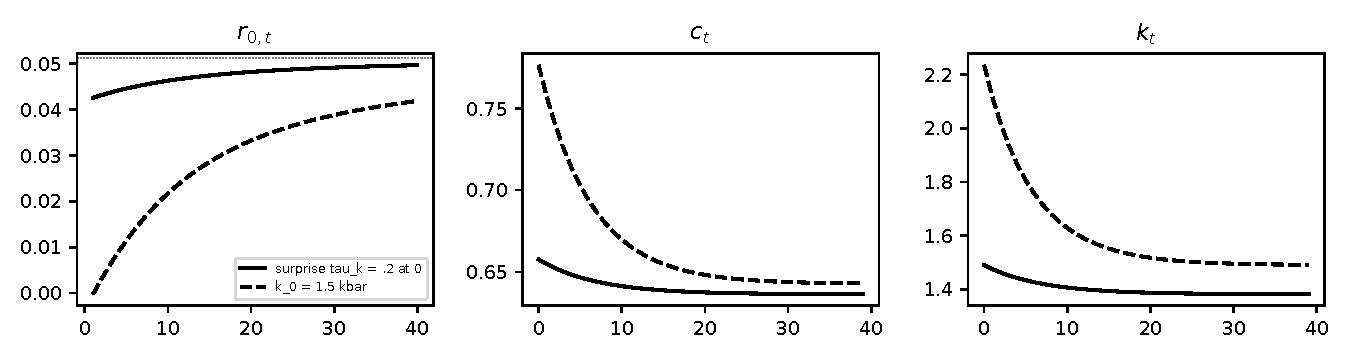
\includegraphics[width=.9\textwidth]{fig/ls11_15_yield_curve.pdf}
\captionof{figure}{Exercise 11.15: yield curves at $t=0$ and the implied paths; surprise $\tau_k$ (solid), $k_0=1.5\kb$
(dashed).}
\end{center}
\end{tcolorbox}

%------- 11.16 -------
\begin{tcolorbox}[evenbox,title={Exercise 11.16 \quad High and low $\gamma$}]
\begin{tcolorbox}[questionbox]
p.~467. The structure of the economy is identical to that described in exercise 11.14. Assume that
$\{g_t,\tau_{ct},\tau_{kt}\}_{t=0}^\infty$ are all constant sequences (their values don't change over time). In this
problem, we ask you to infer differences across two economies in which all aspects of the economy are identical
\emph{except} the parameter $\gamma$ in the utility function. (It is possible that lump sum taxes differ across the two
economies. Assume that lump sum taxes are adjusted to balance the government budget.) In both economies, $\gamma>0$. In one
economy, $\gamma>0$ is high and in the other it is low. Among other identical features, the two economies have identical
government policies and identical initial capital stocks.

\textbf{a.} Please look at figure 11.4. Please tell which outcome for $\{k_{t+1}\}_{t=0}^\infty$ describes the low
$\gamma$ economy, and which describes the high $\gamma$ economy. Please explain your reasoning.

\textbf{b.} Please look at figure 11.5. Please tell which outcome for $\{f'(k_t)\}_{t=0}^\infty$ describes the low
$\gamma$ economy, and which describes the high $\gamma$ economy. Please explain your reasoning.

\textbf{c.} Please plot time paths of consumption for the low $\gamma$ and the high $\gamma$ economies.

\smallskip
\emph{[Figure 11.4: capital rises from the same $k_0$ to the same steady state, slowly in panel (a) and very fast in panel
(b). Figure 11.5: $f'(k_t)$ falls to $\rho+\delta$, slowly in panel (a) and very fast in panel (b).]}
\end{tcolorbox}

\textbf{Solution:} Constant policies give the same steady state $\kb$ for both economies ((11.6.7) does not contain
$\gamma$), the same $\Rb=1+\rho$ and the same $\cb$. They differ only in the speed of the transition. Linearised,
$k_{t+1}-\kb=\lambda_2(k_t-\kb)$, and $\lambda_2$ increases with $\gamma$ (11.7(c), corrected (11.10.16)). Equivalently,
by (11.6.9) a given gap $\Rb_{t+1}-(1+\rho)$ produces consumption growth $\gamma^{-1}\log(\beta\Rb_{t+1})$, large when
$\gamma$ is small.

\textbf{(a)} Panel (a), slow convergence, is the \emph{high}-$\gamma$ economy. Panel (b), fast convergence, is the
\emph{low}-$\gamma$ economy. With low $\gamma$ the household does not mind a steep consumption profile: it sacrifices a lot of
consumption early and invests heavily, so $k$ reaches $\kb$ quickly. With high $\gamma$ it smooths consumption and
accumulates slowly.

\textbf{(b)} $f'$ is decreasing, so $f'(k_t)$ mirrors $k_t$: panel (a), slow decline to $\rho+\delta$, is high $\gamma$;
panel (b), fast decline, is low $\gamma$.

\textbf{(c)} Both consumption paths rise to the same $\cb$. Low $\gamma$: $c_0$ very low (heavy investment), then a steep
rise, close to $\cb$ within a few periods. High $\gamma$: $c_0$ higher, then a slow rise. The paths cross: after a few
periods the low-$\gamma$ economy has more capital and consumes more.

\begin{tcolorbox}[databox]
Benchmark with $g=.2$, $k_0=.5\kb$; $\gamma=.2$ vs $\gamma=5$ ($\lambda_2=.5779$ vs $.9109$). Low $\gamma$:
$k_5=1.4287$, $c_0=.2945$; high $\gamma$: $k_5=.9780$, $c_0=.5071$; consumption paths cross at $t=3$. Newton vs shooting
to $10^{-7}$.
\end{tcolorbox}

\begin{center}
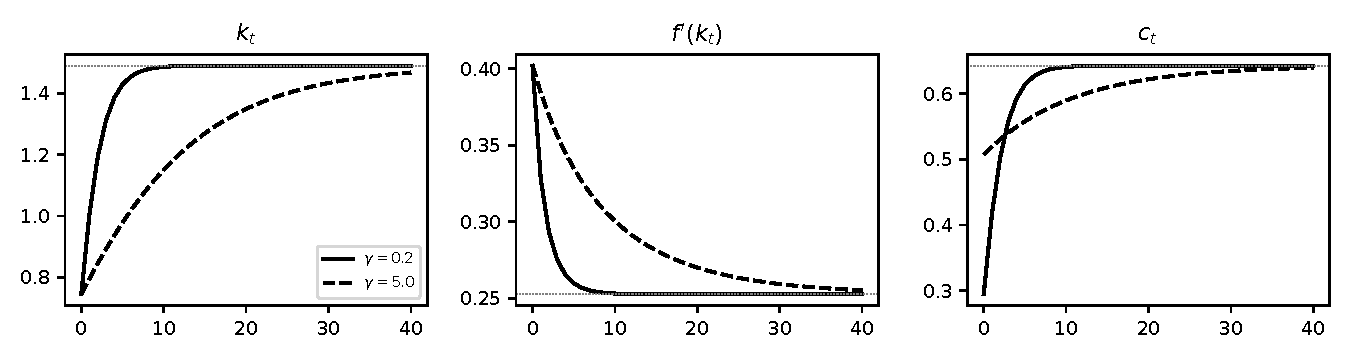
\includegraphics[width=.9\textwidth]{fig/ls11_16_gamma.pdf}
\captionof{figure}{Exercise 11.16: $\gamma=.2$ (solid) vs $\gamma=5$ (dashed); dotted lines: common steady state.}
\end{center}
\end{tcolorbox}

%------- 11.17 -------
\begin{tcolorbox}[oddbox,title={Exercise 11.17 \quad Anticipated vs unanticipated jump in $g$}]
\begin{tcolorbox}[questionbox]
p.~468. The structure of the economy is identical to that described in exercise 11.16. Assume that
$\{\tau_{ct},\tau_{kt}\}_{t=0}^\infty$ are constant sequences (their values don't change over time) but that
$\{g_t\}_{t=0}^\infty$ follows the path described in panel \textbf{c} of figure 11.6 -- it takes a once and for all jump
at time $t=10$. Lump sum taxes adjust to balance the government budget. Panels \textbf{a} and \textbf{b} give consumption
paths for two economies that are identical except in one respect. In one of the economies, the time 10 jump in $g$ had
been anticipated since time 0, while in the other, the jump in $g$ that occurs at time 10 is completely unanticipated at
time 10. Please tell which panel corresponds to which view of the arrival of news about the path of $g_t$. Please say as
much as you can about how $\{k_{t+1}\}_{t=0}^\infty$ and the interest rate behave in these two economies.

\smallskip
\emph{[Figure 11.6: panel a: $c_t\approx.64$ until $t=10$, then a jump down to $\approx.44$ and flat; panel b: $c_t$
declines smoothly from $\approx.6$ toward $\approx.44$; panel c: $g_t=.2$ until $t=10$, then $.4$.]}
\end{tcolorbox}

\textbf{Solution:}

\emph{Panel a: unanticipated.} Before $t=10$ nobody expects a change: the economy stays in the old steady state. At
$t=10$ the permanent, lump-sum-financed rise in $g$ is a pure wealth effect (11.5(c)): consumption falls by exactly
$\Delta g=.2$, and nothing else changes. $k_t=\kb$ throughout and $\Rb_t=1+\rho$, $r_{t,t+1}=-\log\beta$ throughout.

\emph{Panel b: anticipated since 0.} At $t=0$ the present value of lump-sum taxes jumps, so consumption drops at once
(wealth effect) and then keeps declining (section 11.9, figure 11.9.1). The household smooths consumption by building a
stock of capital before $t=10$ and running it down afterwards. So $k$ rises from $\kb$ to a peak at $t=10$ and returns to
$\kb$ (the steady state does not depend on $g$). A declining consumption path needs $\Rb_{t+1}<1+\rho$, by (11.6.9): the
interest rate $r_{t,t+1}=\log\Rb_{t+1}$ falls below $-\log\beta$ from $t=0$, reaches its minimum between 9 and 10 when
$k$ peaks, and rises back afterwards.

\begin{tcolorbox}[databox]
Benchmark, $g=.2\to.4$ at $t=10$. Anticipated: $c_0=.6092$, $c_{10}=.5390$, $c_{40}=.4446$; $k_{10}=2.0985$ (maximum);
minimum $\Rb=\Rb_{10}=1.0008$; $c$ strictly decreasing and $\Rb<1+\rho$ for 40 periods (checked). Surprise: the Newton
path is $k_t=1.4900$, $c=.6426$ before 10 and $.4426$ after, $\Rb=1.0526$ throughout.
\end{tcolorbox}

\begin{center}
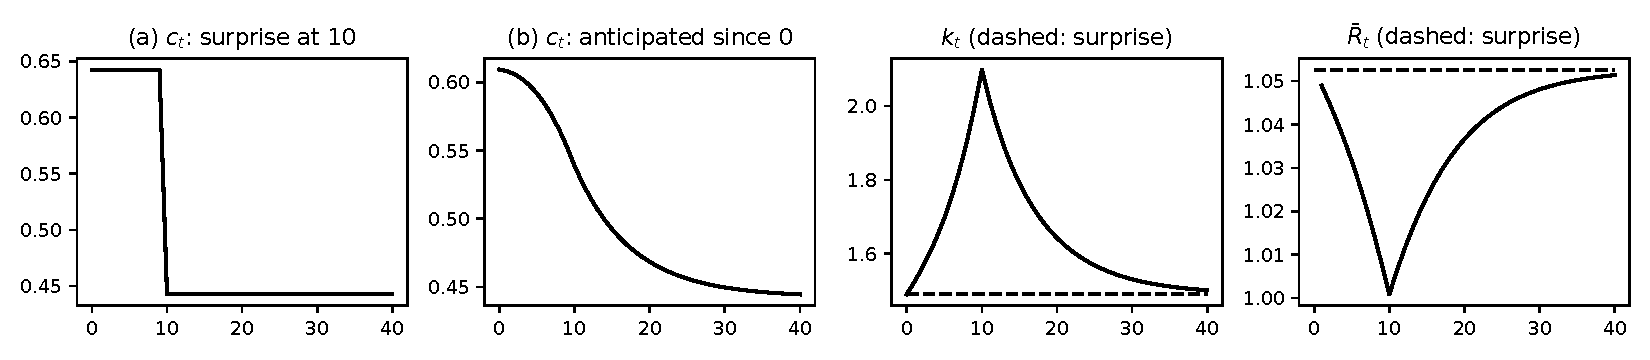
\includegraphics[width=\textwidth]{fig/ls11_17_news.pdf}
\captionof{figure}{Exercise 11.17: panels (a) and (b) reproduced; capital and $\Rb$ under anticipation (solid) and surprise
(dashed).}
\end{center}
\end{tcolorbox}

%----------------------------------------------------------------------
\subsection{Habits, and the Invisible Hand (11.18--11.20)}
%----------------------------------------------------------------------

%------- 11.18 -------
\begin{tcolorbox}[evenbox,title={Exercise 11.18 \quad Habits and durability}]
\begin{tcolorbox}[questionbox]
p.~468. A planner chooses sequences $\{c_t,k_{t+1}\}_{t=0}^\infty$ to maximize
$\sum_{t=0}^\infty\beta^tu(c_t-\alpha c_{t-1})$, $\alpha\in(-1,1)$, $\beta\in(0,1)$ subject to
\[
k_{t+1}+c_t=f(k_t)+(1-\delta)k_t,\quad\delta\in(0,1),\quad c_t\ge0
\]
where $u(x)=\frac{x^{1-\gamma}}{1-\gamma}$ if $\gamma>0$ and $\gamma\ne1$, $\log(x)$ if $\gamma=1$, and $(k_0,c_{-1})$ are
given initial conditions. Here $u'>0$, $u''<0$, and $\lim_{c\downarrow0}u'(c)=0$. If $\alpha>0$, it indicates that the
consumer has a `habit'; if $\alpha<0$, it indicates that the consumption good is somewhat durable.

\textbf{a.} Find a complete set of first-order necessary conditions for the planner's problem.

\textbf{b.} Define an optimal \emph{steady state}.

\textbf{c.} Find optimal steady state values for $(k,f'(k),c)$.

\textbf{d.} For given initial conditions $(k_0,c_{-1})$, describe as completely as you can an algorithm for computing a
path $\{c_t,k_{t+1}\}_{t=0}^\infty$ that solves the planning problem.
\end{tcolorbox}

\textbf{Solution:} \emph{Misprint.} ``$\lim_{c\downarrow0}u'(c)=0$'' should be $+\infty$ (Inada; for the stated $u$,
$u'(x)=x^{-\gamma}\to\infty$). We assume $c_t-\alpha c_{t-1}>0$ along the path.

\textbf{(a)} Lagrangian with multipliers $\beta^t\mu_t$:
\[
\mathcal L=\sum_{t\ge0}\beta^t\big\{u(c_t-\alpha c_{t-1})+\mu_t[f(k_t)+(1-\delta)k_t-c_t-k_{t+1}]\big\}.
\]
$c_t$ appears in $u(c_t-\alpha c_{t-1})$ (date $t$) and in $u(c_{t+1}-\alpha c_t)$ (date $t+1$). FOCs:
\begin{align*}
c_t:&\quad \mu_t=u'(c_t-\alpha c_{t-1})-\alpha\beta\,u'(c_{t+1}-\alpha c_t),\tag{11.18.1}\\
k_{t+1}:&\quad \mu_t=\beta\mu_{t+1}\big[f'(k_{t+1})+1-\delta\big],\tag{11.18.2}\\
&\quad k_{t+1}=f(k_t)+(1-\delta)k_t-c_t,\tag{11.18.3}
\end{align*}
for $t\ge0$, with $(k_0,c_{-1})$ given and the transversality condition $\lim_t\beta^t\mu_tk_{t+1}=0$. $\mu_t$ is the
marginal value of goods at $t$: one more unit consumed raises utility today but, through the habit, lowers utility
tomorrow ($\alpha>0$), or raises it through durability ($\alpha<0$).

\textbf{(b)} An optimal steady state is a triple $(k,c,\mu)$ that satisfies (11.18.1)--(11.18.3) with $k_t=k$, $c_t=c$,
$\mu_t=\mu$ for all $t$. If $(k_0,c_{-1})=(k,c)$, the optimal plan stays there.

\textbf{(c)} (11.18.2): $1=\beta[f'(k)+1-\delta]$, so $f'(\kb)=\rho+\delta$; (11.18.3): $\cb=f(\kb)-\delta\kb$;
(11.18.1): $\mu=(1-\alpha\beta)u'((1-\alpha)\cb)>0$ (because $|\alpha|<1$). The steady state $(\kb,f'(\kb),\cb)$ is the same
as without habits: habits and durability change the dynamics, not the long run.

\textbf{(d)} Substituting (11.18.1) into (11.18.2) gives one equation in consumption at four dates and capital:
\[
u'(c_t-\alpha c_{t-1})-\alpha\beta u'(c_{t+1}-\alpha c_t)=\beta[f'(k_{t+1})+1-\delta]\big[u'(c_{t+1}-\alpha c_t)-\alpha\beta
u'(c_{t+2}-\alpha c_{t+1})\big].
\]
With (11.18.3), the system maps $s_t=(k_t,c_{t-1},c_t,c_{t+1})$ into $s_{t+1}$: solve (11.18.3) for $k_{t+1}$, then the
equation above for $c_{t+2}$. Two components are predetermined, $(k_0,c_{-1})$, and two are free, $(c_0,c_1)$; the
terminal condition requires convergence to $(\kb,\cb)$. Algorithms:
\begin{enumerate}[label=\arabic*.]
\item \emph{Newton on the whole path} (used here). Pick $S$ large. Unknowns $k_1,\dots,k_S$, with $k_{S+1}=k_{S+2}=\kb$;
$c_t=Y(k_t)-k_{t+1}$ for $t=0,\dots,S+1$, $c_{-1}$ given. Impose the Euler equation for $t=0,\dots,S-1$: $S$ equations in
$S$ unknowns. Each equation involves $k_{t-1},\dots,k_{t+3}$, so the Jacobian is banded and cheap.
\item \emph{Two-dimensional shooting}: guess $(c_0,c_1)$, iterate $s_{t+1}=F(s_t)$ forward, and adjust the guesses (by
Newton on two unknowns; bisection no longer applies) until $(k_S,c_S)\approx(\kb,\cb)$.
\item \emph{Linear approximation}: linearise $F$ at the steady state, $\hat s_{t+1}=J\hat s_t$. Generically $J$ has two
roots inside and two outside the unit circle, in pairs $(\lambda,1/(\beta\lambda))$ as in section 11.10.1. Choose
$(\hat c_0,\hat c_1)$ so that $\hat s_0$ lies in the span of the stable eigenvectors, given $(\hat k_0,\hat c_{-1})$; then
$\hat s_t=V_s\Lambda_s^tw$ (solving stable roots backward and unstable roots forward).
\end{enumerate}

\begin{tcolorbox}[databox]
$\gamma=2$, benchmark $f$, $g=0$; the book's habit parameter is written $a$ in the code. Steady state
$\kb=1.489956$, $f'(\kb)=.252632$, $\cb=.842645$ for every $a$; $\mu=2.9575$ ($a=.5$), $1.0709$ ($a=-.3$).
Eigenvalues of $J$: $a=.5$: $.5162,.8219,1.2807,2.0390$; $a=-.3$: $-3.5581,-.2958,.8309,1.2668$. The negative pair makes
consumption oscillate when the good is durable. Pairing $\lambda\cdot1/(\beta\lambda)$ checked. Newton vs the stable-subspace
solution for $k_0=.99\kb$, $c_{-1}=\cb$: max $|\Delta k|=1.2\times10^{-5}$ ($a=.5$), $6.4\times10^{-6}$ ($a=-.3$), against a
deviation of $.0149$. At $a=0$ the Newton path equals the standard model's.
From $k_0=.5\kb$, $c_{-1}=f(k_0)-\delta k_0=.7584$: $c_0=.6475$ ($a=0$), $.7018$ ($a=.5$: habit keeps consumption close to
$c_{-1}$ and slows accumulation, $k_{10}=1.3428$ vs $1.3602$), $.6158$ ($a=-.3$: consumption zig-zags, $.6158,.7012,.7120,\dots$).
\end{tcolorbox}

\begin{center}
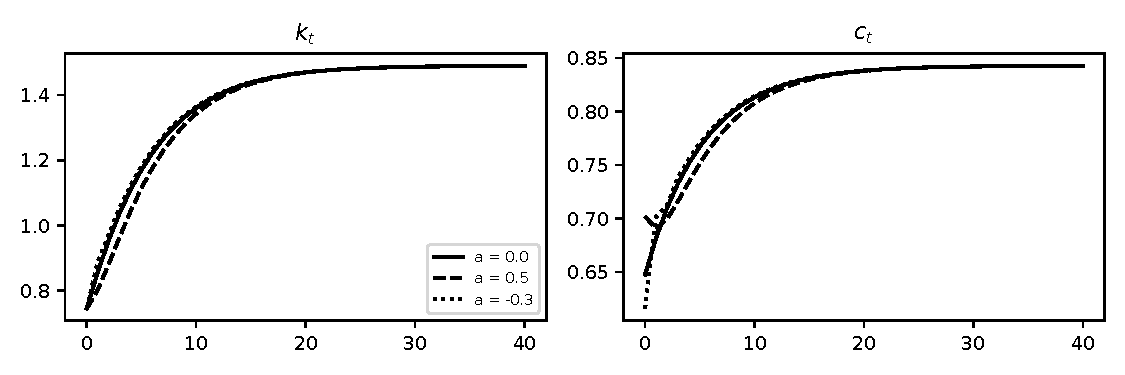
\includegraphics[width=.8\textwidth]{fig/ls11_18_habit.pdf}
\captionof{figure}{Exercise 11.18: paths from $k_0=.5\kb$ for $a=0$ (solid), habit $a=.5$ (dashed), durability
$a=-.3$ (dotted).}
\end{center}
\end{tcolorbox}

%------- 11.19 -------
\begin{tcolorbox}[oddbox,title={Exercise 11.19 \quad The invisible hand, I}]
\begin{tcolorbox}[questionbox]
p.~469. Please consider once again the ``Foreseen jump in $g$'' experiment studied in section 11.9. This exercise asks you
to put yourself in the shoes of the representative household and to think through the optimum problem that it faces
within a competitive equilibrium at time 0.

\textbf{a.} Please describe the signals that the market sends to the household \emph{after} the new
$\{g_t\}_{t=0}^\infty$ policy materializes at time 0. Please list all of the objects that ``the market'' (also known as
``the invisible hand'') presents as \emph{exogenous} to the representative household.

\textbf{b.} Please describe how the ``Big $K$'' part of a ``Big $K$, little $k$'' argument is used to determine
\emph{all} of those objects exogenous to the household. \textbf{Hint:} This is accomplished by applying the shooting
algorithm in section 11.9.

\textbf{c.} Please explain thoroughly how the representative household chooses to respond to the signals presented to it
by the market at time 0.

\textbf{d.} Given the objects that the market presents to the representative household, please tell how you would could a
shooting algorithm to compute the path of $\{c_t,k_{t+1}\}_{t=0}^\infty$ chosen by the household.

\textbf{e.} Please describe how to complete a ``Big $K$, little $k$'' argument using your answers to parts \textbf{c}
and \textbf{d}.
\end{tcolorbox}

\textbf{Solution:} Experiment: benchmark economy at its steady state; at $t=0$ it becomes known that $g$ rises from $.2$ to
$.4$ at $t=10$, financed by lump-sum taxes.

\textbf{(a)} The household does not need to observe $g_t$. It sees: the time-0 price system $\{q_t,\eta_t,w_t\}_{t\ge0}$
(prices of dated goods, rental rates, wages) and its tax bill $\{\tau_{ht}\}_{t\ge0}$ (only $\sum_tq_t\tau_{ht}$ matters),
with distorting taxes at zero. Exogenous to the household: $\{q_t,\eta_t,w_t,\tau_{ht}\}$ and its own $k_0$. The news
reaches it only through these objects: a higher present value of taxes and a new shape of $q_t$ (lower interest rates).

\textbf{(b)} Big $K$: the economist (or the invisible hand) solves for the aggregate path $\{K_{t+1}\}$ by shooting on the
aggregate Euler equation and feasibility,
\[
u'(C_t)=\beta u'(C_{t+1})[f'(K_{t+1})+1-\delta],\qquad C_t=f(K_t)+(1-\delta)K_t-g_t-K_{t+1},
\]
from $K_0=\kb$ toward $\kb$ with the new $\{g_t\}$. It then sets prices from (11.6.8):
$q_t=\beta^tu'(C_t)/u'(C_0)$, $\eta_t=f'(K_t)$, $w_t=f(K_t)-K_tf'(K_t)$, and taxes with
$\sum_tq_t\tau_{ht}=\sum_tq_tg_t$ (e.g.\ $\tau_{ht}=g_t$).

\textbf{(c)} Household problem at those prices: $\max\sum_t\beta^tu(c_t)$ s.t.
$\sum_tq_t[c_t+k_{t+1}-(1-\delta)k_t]\le\sum_tq_t[\eta_tk_t+w_t-\tau_{ht}]$. Because the prices satisfy no arbitrage,
$q_{t-1}=q_t(\eta_t+1-\delta)$, the coefficient of every $k_t$, $t\ge1$, is zero. The household is indifferent about how it
holds its wealth, and the budget collapses to
\[
\sum_tq_tc_t\le W_0\equiv q_0(\eta_0+1-\delta)k_0+\sum_tq_t(w_t-\tau_{ht}).
\]
FOC $\beta^tu'(c_t)=\mu q_t$ gives $c_t=(\mu q_t/\beta^t)^{-1/\gamma}$, and the budget pins down $\mu$:
$\mu^{-1/\gamma}\sum_tq_t(q_t/\beta^t)^{-1/\gamma}=W_0$. The response has two parts. \emph{Wealth}: higher $\tau_h$ lowers
$W_0$ and scales every $c_t$ down. \emph{Tilt}: $q_t/\beta^t$ rises over $t\le10$ (interest rates below $\rho$), so $c_t$
declines over time. Its capital holdings follow from the period budget once the timing of taxes is fixed.

\textbf{(d)} Shooting at \emph{given} prices: guess $c_0$; iterate $u'(c_{t+1})=u'(c_t)\,q_{t+1}/(\beta q_t)$ and
$k_{t+1}=(\eta_t+1-\delta)k_t+w_t-\tau_{ht}-c_t$ (with $\tau_{ht}=g_t$); raise $c_0$ if $k_S$ ends above the target and lower
it if below, until $k_S\approx\kb$ (equivalently, until the present-value budget holds with equality). Unlike the
algorithm of (b), the prices do not respond to the household's $k$.

\textbf{(e)} The prices of (b) are equilibrium prices if the household's optimal choices at those prices, from (c)--(d),
reproduce the aggregates: $c_t=C_t$ and $k_t=K_t$ for all $t$. Then markets clear and every agent optimises. This holds
here because the aggregate Euler equation of (b) \emph{is} the household's Euler equation evaluated at $c=C$, $k=K$:
the shooting in (b) finds the fixed point of the map from a conjectured aggregate law of motion to the household's
choices.

\begin{tcolorbox}[databox]
Big $K$ by Newton; little $k$ in closed form at those prices: $\mu=2.694141$ (with $q_0=1$); household $c_0=.609242=C_0$;
$c_t=C_t$ to $10^{-6}$ relative for all $t$; $k_t=K_t$ over 60 periods to $2.8\times10^{-10}$ (with $\tau_{ht}=g_t$);
no-arbitrage $q_t/q_{t+1}=\eta_{t+1}+1-\delta$ checked.
\end{tcolorbox}
\end{tcolorbox}

%------- 11.20 -------
\begin{tcolorbox}[evenbox,title={Exercise 11.20 \quad The invisible hand, II}]
\begin{tcolorbox}[questionbox]
p.~470. Please consider again the ``Foreseen jump in $\tau_n$'' experiment in section 11.12. Like the previous problem,
this one puts you into the shoes of the representative household and asks you to think through the optimum problem that
it faces within a competitive equilibrium with distorting taxes at time 0.

\textbf{a.} Please describe the signals that the market sends to the household \emph{after} the new
$\{\tau_{nt}\}_{t=0}^\infty$ policy materializes at time 0. Please list all objects that ``the market'' presents as
\emph{exogenous} to the representative household.

\textbf{b.} Keeping in mind that there is a ``Big $K$, little $k$'' argument in the background, please provide a complete
explanation for why the household chooses the paths of $\{c_t,n_t,k_t\}_{t=0}^\infty$ displayed in figure 11.12.3.
\end{tcolorbox}

\textbf{Solution:} Section 11.12: $U=\ln c+B(1-n)$, $B=3$, $F=k^\alpha n^{1-\alpha}$, $g=.2$, $\tau_c=\tau_k=0$; at $t=0$
it becomes known that $\tau_n$ rises from 0 to $.2$ at $t=10$; lump-sum transfers balance the budget.

\textbf{(a)} The household sees the price system $\{q_t,\eta_t,w_t\}_{t\ge0}$, the announced labour-tax path
$\{\tau_{nt}\}$ (0 for $t\le9$, $.2$ after), $\tau_{ct}=\tau_{kt}=0$, and its lump-sum taxes or transfers $\{\tau_{ht}\}$
(through their present value). These, with $k_0$, are exogenous to it.

\textbf{(b)} Household problem:
$\max\sum_t\beta^t[\ln c_t+B(1-n_t)]$ s.t. $\sum_tq_t[c_t+k_{t+1}-(1-\delta)k_t]\le\sum_tq_t[\eta_tk_t+(1-\tau_{nt})w_tn_t-\tau_{ht}]$.
FOCs:
\[
\frac{\beta^t}{c_t}=\mu q_t,\qquad \beta^tB=\mu q_t(1-\tau_{nt})w_t\quad(0<n_t<1),\qquad
\frac{q_t}{q_{t+1}}=1+\eta_{t+1}-\delta .
\]
Dividing: $Bc_t=(1-\tau_{nt})w_t$ (11.12.15c), and $c_{t+1}=\beta\Rb_{t+1}c_t$ (11.12.15a).
\emph{Key feature}: utility is linear in leisure. At prices that satisfy these conditions, the marginal value of an hour of work
is the same at every date, so the household is indifferent about \emph{when} it works; only the present value of its labour
income matters. Its consumption is pinned down by the after-tax wage, and its hours and capital are pinned down by market
clearing, i.e.\ by the Big $K$ path. The figure then follows:
\begin{itemize}[itemsep=2pt]
\item \emph{Long run.} (11.12.12) fixes $k/n=\tilde k$ independently of $\tau_n$, so the pre-tax wage returns to its old
value, and $c=(1-\tau_n)w/B$ falls by $20\%$. By (11.12.14) $n$ falls, and $k=\tilde kn$ falls with it.
\item \emph{Before $t=10$.} Work is cheap in utility terms relative to after 10: the after-tax wage is high now and will be
low later. The household works more before 10 ($n$ rises) and invests the extra output ($k$ rises): intertemporal
substitution of labour. Consumption stays essentially at its old level. By the Euler equation and $Bc_t=w_t$, a flat $c$
requires a constant $\Rb$ and wage, i.e.\ a constant $k/n$, so $k$ and $n$ rise together. (Exactly, $c_t$ is a hair below
its old level and rises toward it: $c_{t+1}=\beta\Rb(\kappa(c_{t+1}))c_t$ with $\kappa$ increasing in $c$ is a stable map
toward $\cb$.)
\item \emph{At $t=10$.} Hours drop sharply. The capital built up raises $k/n$ and the pre-tax wage, so the after-tax wage
falls by less than $20\%$ at first. $\Rb_{10}$ falls below 1 (low $f'$ at a high $k/n$), so consumption falls.
\item \emph{After $t=10$.} Capital is run down, $k/n$ falls back to $\tilde k$, the wage declines to its old value, $\Rb$
rises back to $1+\rho$, $c$ declines to its new level and $n$ recovers to its new, lower steady state.
\end{itemize}
Big $K$, little $k$: the particular paths of $n_t$ and $k_t$ are those that, aggregated, generate the prices at which the
household is willing to supply them.

\begin{tcolorbox}[databox]
Old steady state $k=.8041$, $c=.2547$, $n=.5397$; new $k=.7140$, $c=.2038$, $n=.4792$. Before 10, $c_t/c_{\rm old}-1\in
[-1.15\times10^{-3},-3.2\times10^{-5}]$; $n_9=.6136$, $k_{10}=.9764$, $n_{10}=.4087$, $w_{10}=.8931$, $\Rb_{10}=.9841$
(figure 11.12.3 reproduced). Newton on (11.12.15) vs shooting on $c_0$ (solving for $k_{t+1}/n_{t+1}$ each period): paths
agree to $10^{-7}$; $Bc_t=(1-\tau_{nt})w_t$ holds on the path.
\end{tcolorbox}

\begin{center}
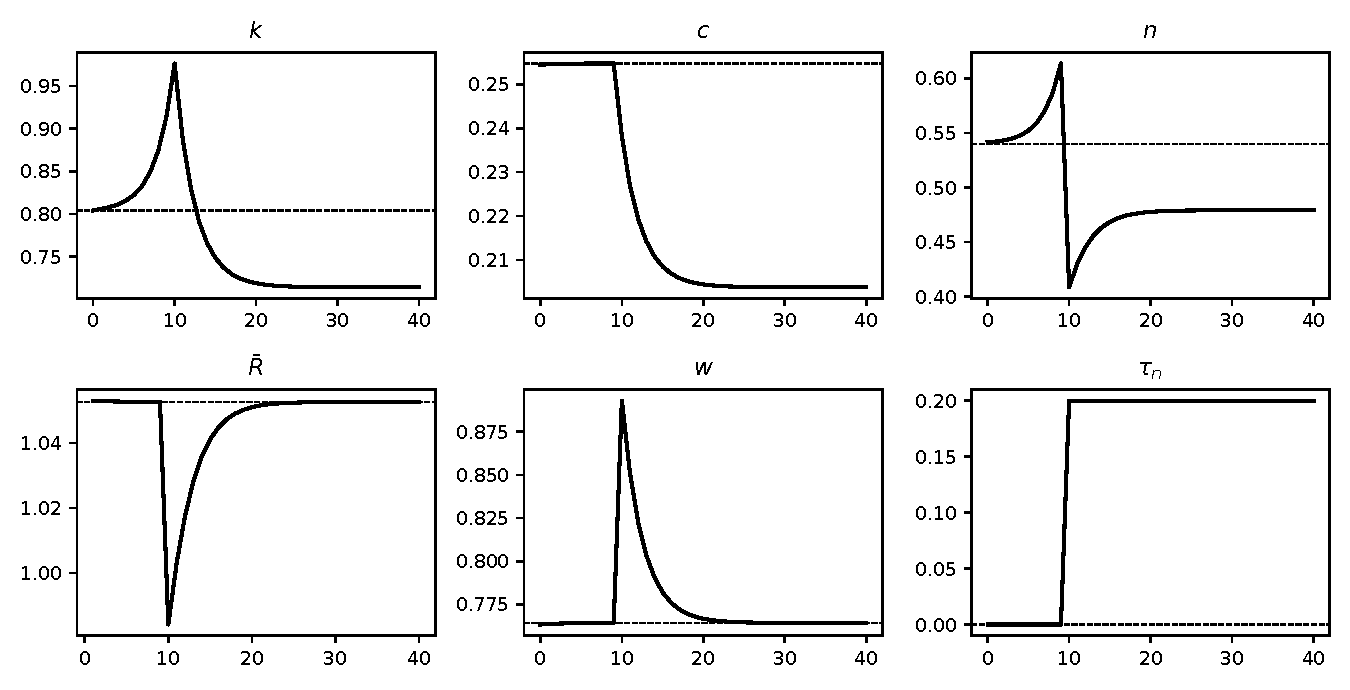
\includegraphics[width=.9\textwidth]{fig/ls11_20_tau_n.pdf}
\captionof{figure}{Exercise 11.20: response to the foreseen rise in $\tau_n$ at $t=10$ (dashed: old steady state).}
\end{center}
\end{tcolorbox}

%======================================================================
\section*{Companion code}
\addcontentsline{toc}{section}{Companion code}
%======================================================================

Every numerical result above is reproduced by the notebook \texttt{ls\_ch11.ipynb} in this folder
(executed, outputs saved). Each claim is checked by an independent route with an \texttt{assert}.

\begin{center}
\begin{tabular}{@{}lp{11.2cm}@{}}
\toprule
\textbf{Section} & \textbf{What it checks} \\
\midrule
Shared & Policy paths $(g,\tau_c,\tau_k,\psi,\text{levy})$; damped Newton with banded finite-difference Jacobian on (11.6.3);
shooting of section 11.6.3 by bisection on $c_0$; linearisation (11.10.8) from numerical derivatives of $H$; prices (11.6.8).
The ch.~5/7 LQ toolkit is not needed. \\
11.1--11.4 & Newton vs shooting; PV budgets by \texttt{brentq}; Laffer curves (steady-state $\tau_k$; levy at $T=10$);
sequential government budget (11.4.2). \\
11.5--11.9 & Flat paths after a surprise $g$; open-economy budgets; welfare rankings; linear vs Newton (error first order);
$\lambda_2$ root vs corrected (11.10.16); \texttt{linprog} corners. \\
11.10--11.17 & $r_{t,t+1}=\log\Rb_{t+1}$; shapes (monotonicity, concavity) of $c$, $k$, $\Rb$, $r_{0,t}$; VFI vs closed form;
revenue-neutral $\bar\tau_k$. \\
11.18--11.20 & Habit Newton vs stable subspace, root pairing; household problem at equilibrium prices vs aggregates;
elastic-labour Newton vs shooting. \\
\bottomrule
\end{tabular}
\end{center}

Figures are saved to \texttt{fig/ls11\_*.pdf} with TrueType (not Type~3) fonts.

\end{document}
